\section{Architectural Design}
\subsection{Overview}
In Figure \ref{fig:three_layers_application} it's present the black-box view of our architecture, that is defined by three different layers represented:

\begin{itemize}
    \item \textbf{Presentation Layer:} it's the layer that is used to present data to the application layer in an accurate, well-defined and standardized format.
    \item \textbf{Application Layer:} it's the layer that manages all the functions that controls the business logic of our system.
    \item \textbf{Data Layer:} it controls how the data are stored and accessed.
\end{itemize}

\begin{figure}[h!]
        \centering
        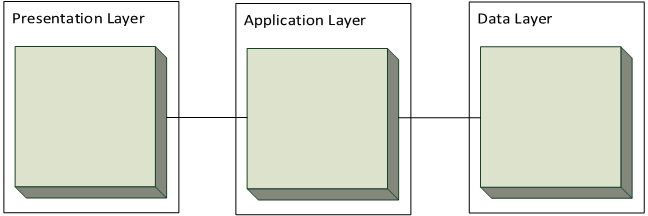
\includegraphics[scale=0.6]{images/three_layers.png}
        \caption{Three layers application}
        \label{fig:three_layers_application}
\end{figure}
\FloatBarrier

A more detailed view of the selected architecture is present in Figure \ref{fig:architecture}:

\begin{figure}[h!]
        \centering
        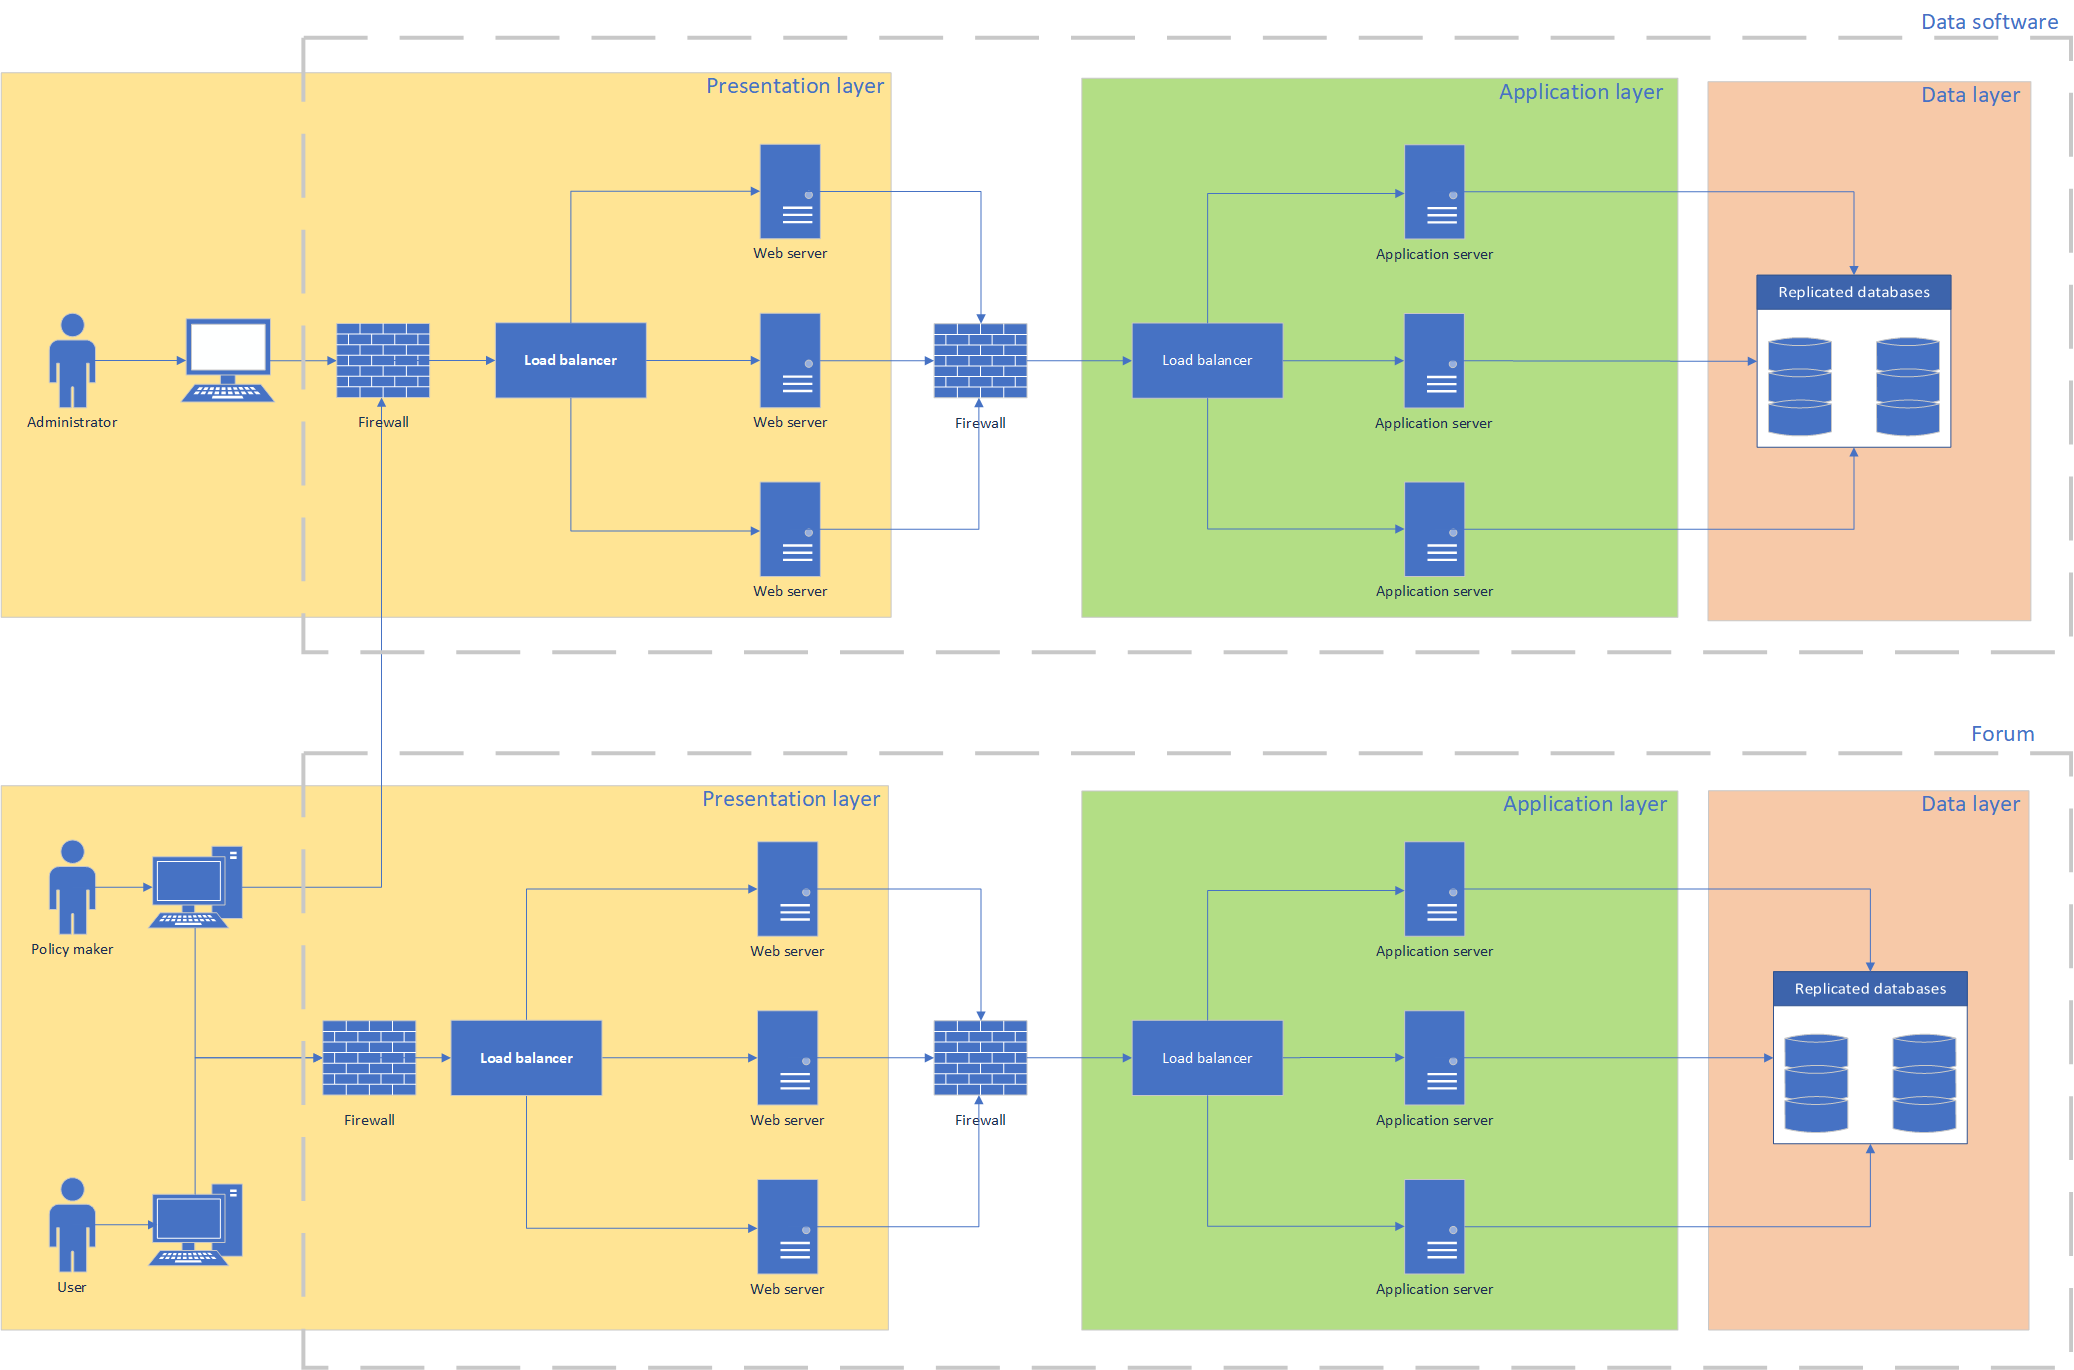
\includegraphics[scale=0.25]{images/architecture_diagram.png}
        \caption{Architecture}
        \label{fig:architecture}
\end{figure}
\FloatBarrier

The service is supposed to be web responsive and for this reason it should be accessible from the vast majority of device from the users. A client-side scripting paradigm will be adopted.

Generally, the architecture divide the application in three different layers: the user can interface with the browser which is connected to replicated Web Servers that act as middleware, while the last layer is represented by the application servers that contain all the application logic. The DBMS APIs provide the function to retrieve and store the data by the application servers.

The nodes are separated by firewalls to guarantee a higher level of security to the system.

The forum and the data aggregator are two different applications and for this reason they will have two distinct back-end and will use different databases. While Administrator can access only to the data aggregator context and the User can enter only in the forum, the Policy makers have access to both area. \\In the following section will be described more in depth the components present in the system.
\newpage
\subsection{Component View}

\begin{figure}[h!]
        \centering
        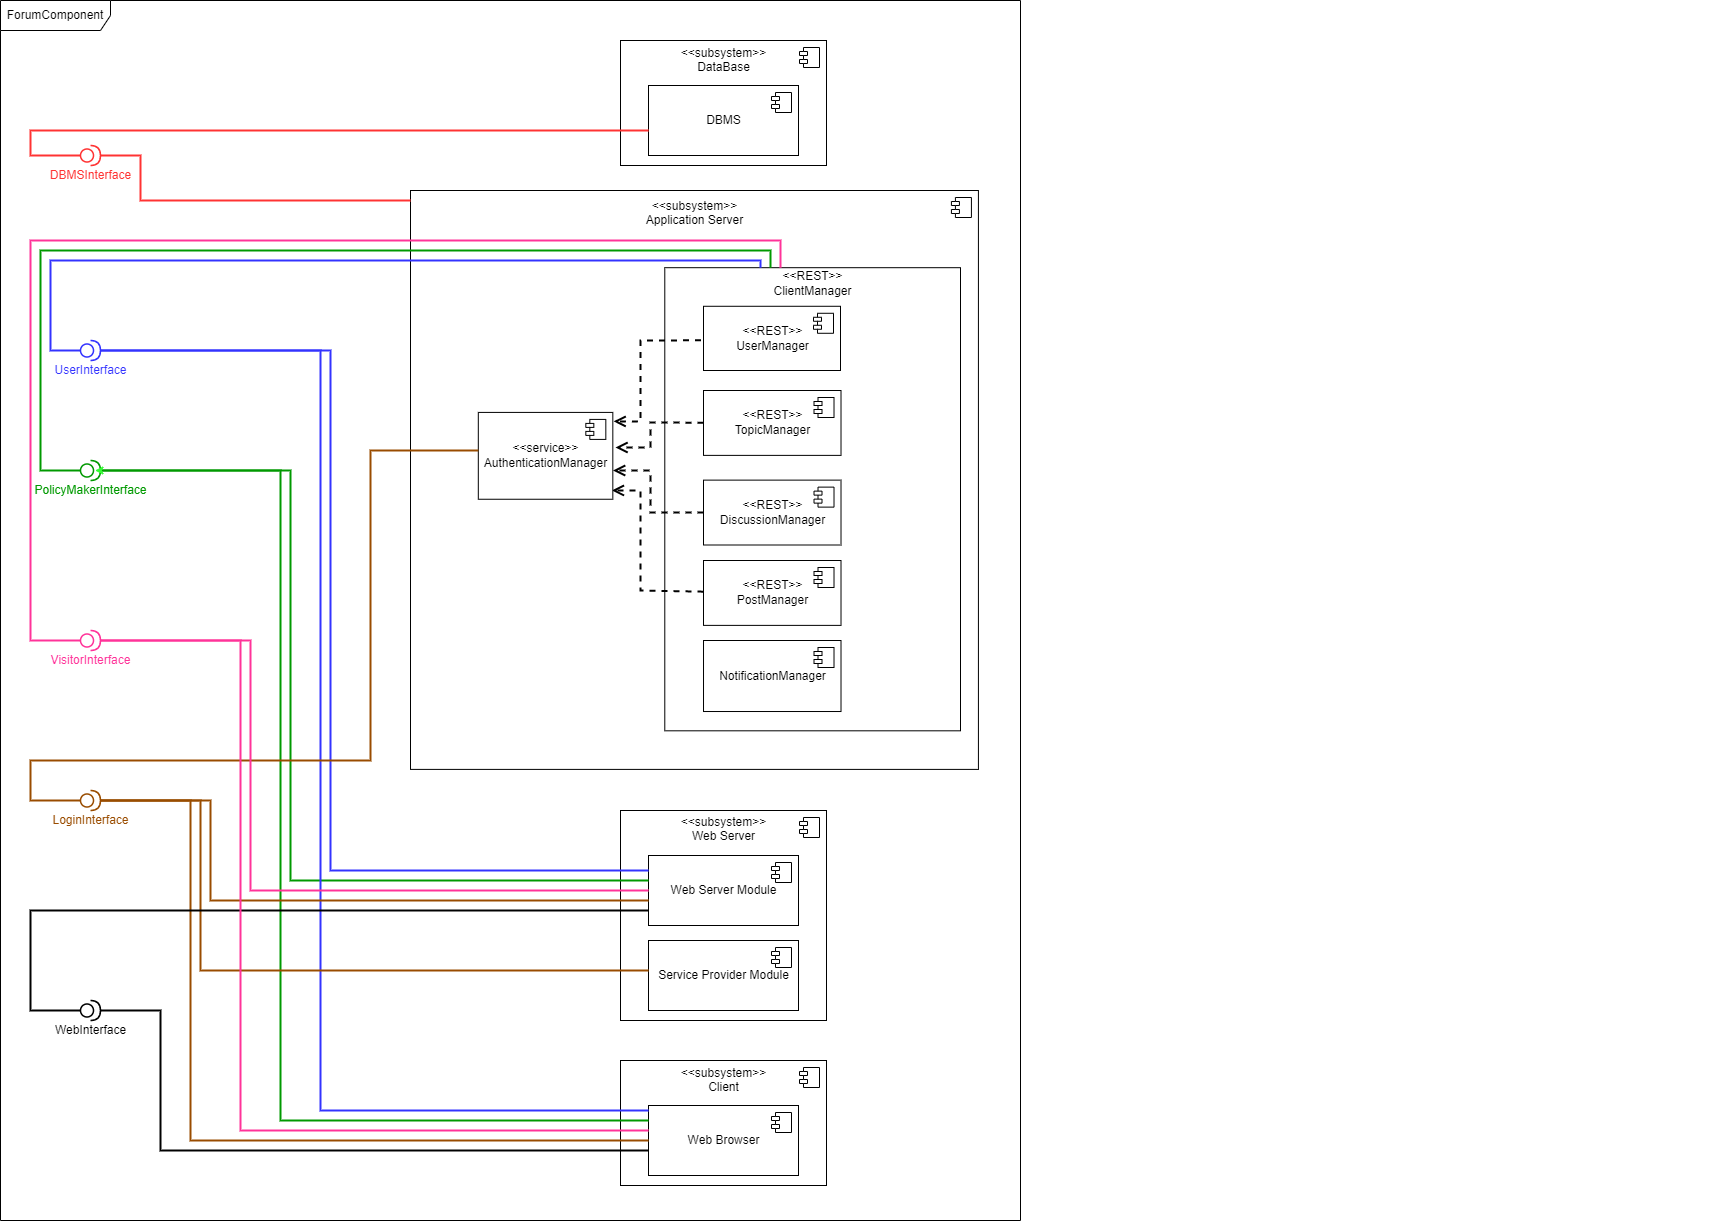
\includegraphics[scale=0.40]{images/component_diagrams/forum_component_diagram.png}
        \caption{Forum Component Diagram}
        \label{fig:forum_component_diagram}
\end{figure}
\FloatBarrier
In figure \ref{fig:forum_component_diagram} is present a complete diagram representing the layers described before, regarding the forum application.
The web server contains two modules:
\begin{itemize}
    \item \textbf{The Web Server Module} is responsible for the web browser request routing, by sending them to the application server, receiving them and sending back responses.
    \item \textbf{The Service Provider Module} generates signed authentication requests to the IdP and receives signed assertion back in order to authenticate the user in the web server session.
\end{itemize}
Instead, the application server contains different modules:
\begin{itemize}
    \item \textbf{AuthenticationManager}\\
    It is responsible for managing user authentication and permissions. It is responsible for authenticating the user after reading the session attributes generated by the service provider and then for creating the logged user session (through the LoginInterface). It is also responsible for filtering each incoming request in order to determine if a user has or not the permission for the requested resource. Finally, it is also in charge of detecting if an unauthenticated user is trying to access a resource redirecting it to the service provider module.
    
    \item \textbf{ClientManager}\\
    This module manages the requests made by the client. When the user is logged in it provides a UserInterface (if the authenticated person is a User) or a PolicyMakerInterface (if the authenticated person is a Policy maker), exposing functions to manage the entity related information (through the UserManager) and the forum content (TopicManager, DiscussionManager and PostManager).\\
    In addition the VisitorInterface provides free access to all Visitor in order to get public content.
    
    \item \textbf{UserManager}\\
    This module provides the functions related to a User, for instances the possibility to retrieve his own replies or his own information.
    
    \item \textbf{TopicManager}\\
    This module provides all the functionalities related to the topics present in the forum, the authorization is managed by the AuthenticationManager Module.
    
    \item \textbf{DiscussionManager}\\
    This module provides all the functionalities related to the discussions present in the forum, the authorization is managed by the AuthenticationManager Module.
    
    \item \textbf{PostManager}\\
    This module provides all the functionalities related to the posts present in the forum, the authorization is managed by the AuthenticationManager Module.
    
    \item \textbf{NotificationManager}\\
    This module handles the email notifications, such as for the publication of a new post or the notification of an approved post.
\end{itemize}
\begin{figure}[h!]
        \centering
        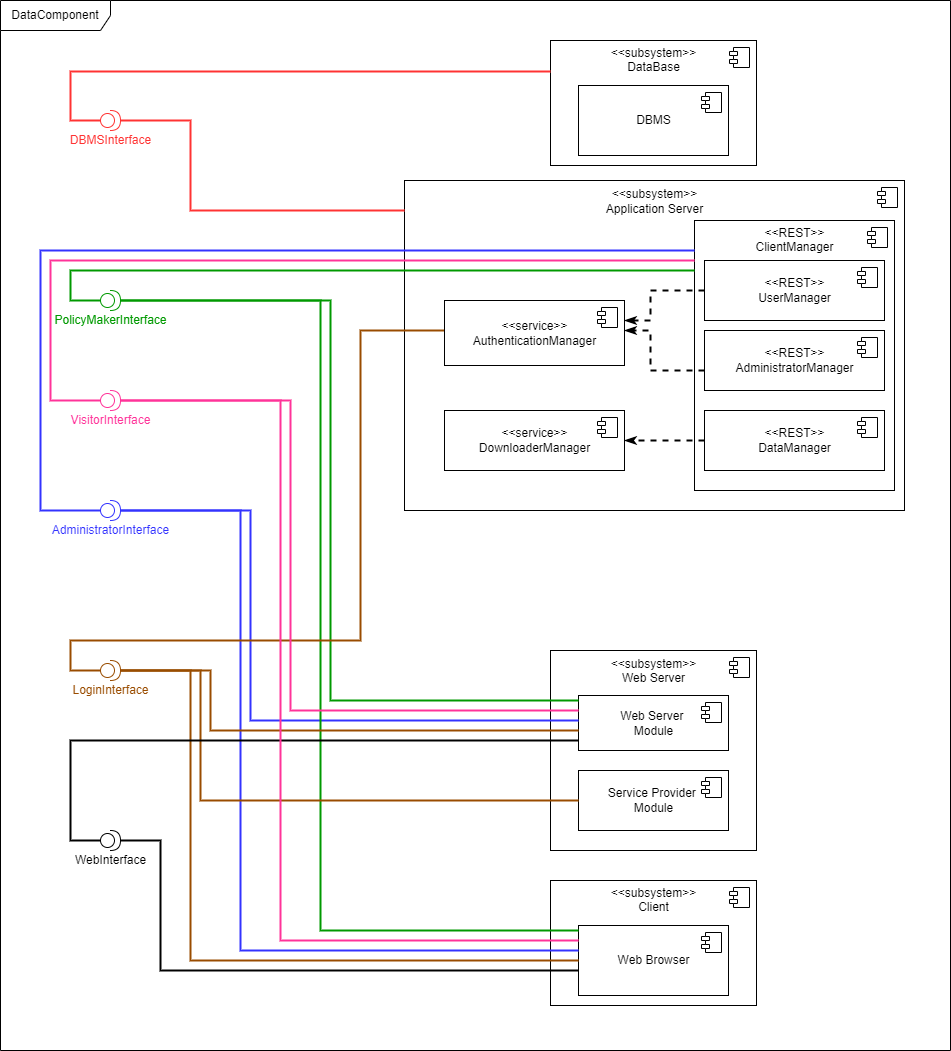
\includegraphics[scale=0.40]{images/component_diagrams/data_component_diagram.png}
        \caption{Data Component Diagram}
        \label{fig:data_component_diagram}
\end{figure}
\FloatBarrier
In figure \ref{fig:data_component_diagram} is present a complete diagram representing the layers described before regarding data aggregator application.\\
The web server contains two modules:
\begin{itemize}
    \item \textbf{The Web Server Module} is responsible for web browser request routing sending them to the application server, receiving and sending back responses.
    \item \textbf{The Service Provider Module} generates signed authentication requests to the IdP and it receives signed assertion back in order to authenticate the user in the web server session.
\end{itemize}
The application server contains different modules:
\begin{itemize}
    \item \textbf{AuthenticationManager}\\
    It is responsible for managing user authentication and permissions. It is in charge of authenticating the user after reading the session attributes generated by the service provider and then to create the logged user session. Then, it is also responsible for filtering each incoming request to determine if a user whether or not has the permission to the requested resource. It is also responsible for detecting if an unauthenticated user is trying to access a resource redirecting it to the Service Provider Module.
    Finally, it manages Administrators login exposing the LoginInterface.
    
    \item \textbf{ClientManager}\\
    This module manages the requests made by the client. The AdministratorInterface is accessed by Administrators and provides functionalities to add, remove and manage data sources (DataManager and DownloaderManager) while the PolicyMakerInterface provides functionalities to get, analyze and recalculate deviance through the DataManager. Both the type of authenticated people have their own Manager (AdministratorManager and UserManager for the Policy makers) that provides functionalities related to the entity (e.g. personal information).
    
    \item \textbf{AdministratorManager}\\
    This module provides the functions related to an Administrator, for instance the possibility to add and remove other Administrators.
    
    \item \textbf{DataManager}\\
    This module provides all the functionalities related to the data management such as add and remove a data source but also to obtain and filter present data.
    
    \item \textbf{DownloaderManager}\\
    This module is responsible for connecting and fetching periodically new data from public data sources, filter and store them. 

\end{itemize}

\newpage
\subsection{Deployment View}

\begin{figure}[h!]
        \centering
        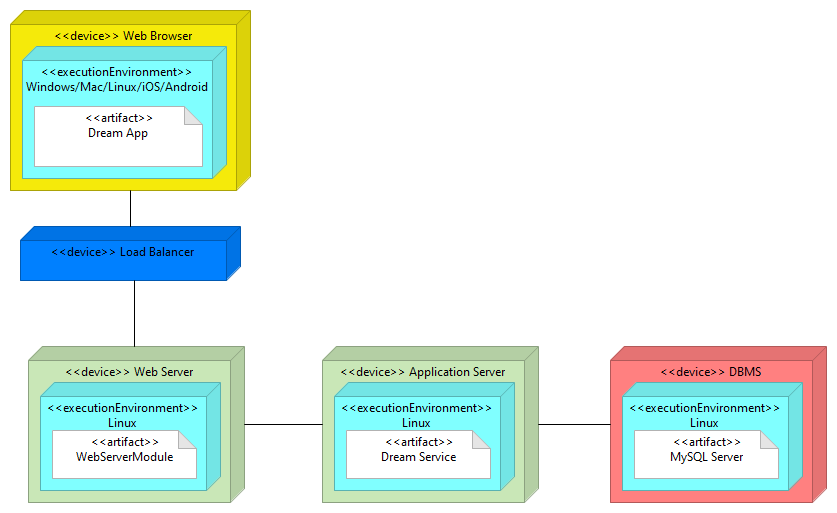
\includegraphics[scale=0.40]{images/deployment_view.png}
        \caption{Deployment Diagram}
        \label{fig:deployement_diagram}
\end{figure}
\FloatBarrier

The deployment diagram in figure \ref{fig:deployement_diagram} shows the topology of the system's hardware and specify the distribution of components. For each device its Operating System is indicated.
\begin{itemize}
    \item \textbf{Tier 1}: It is the client machine. It could be any device provided with a Web Browser running on Windows, Mac or Linux for desktop devices or in iOS or Android for mobile devices.
    \item \textbf{Tier 2}: It consists of the load balancer and the replicated web servers. The first one is a device that allows to balance the workload between servers, to maintain their capacity at an optimal level. This enables a server cluster to handle peak traffic, and provides a backup solution in the event of an outage.
    \\Replicated web servers display website content through storing, processing and delivering web pages to users. They do not execute any business logic but only respond to client requests made over the World Wide Web. They also contains the styling logic of the page.
    \item \textbf{Tier 3}: it consists of the application servers. They provides all the business logic, allowing to communicate to the client tier using APIs and connect to the data tier using the DBMS gateway.
    \item \textbf{Tier 4}: it consists of the database management system servers. The data are stored in those replicated devices and they provide to the application server tier the operations needed to manage the data.
\end{itemize}
\subsection{Runtime View}

\subsubsection{Visitor filters data}

\begin{figure}[h!]
        \centering
        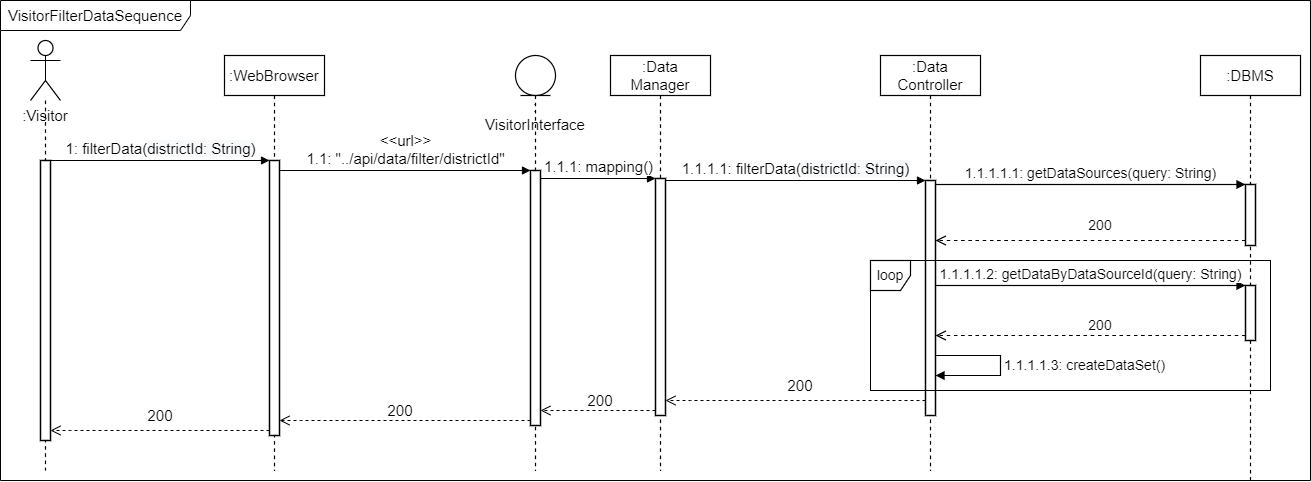
\includegraphics[scale=0.30]{images/runtime_view/visitor_filter_data_runtime_view_diagram.png}
        \caption{Visitor filters data sequence diagram}
        \label{fig:visitor_filters_data_sequence_diagram}
\end{figure}
\FloatBarrier

A Visitor can accesses to the data provided by the platform. In order to consult them more clearly, the visitor can select different filters that allow viewing only the data of interest.\\
Once he has selected the parameters of interest he clicks on the "Filter" button; at this point the Web Browser sends the data to the DataManager through the VisitorInterface doing a GET to "../api/data/filter/\{districtId\}" (where districtId is the id of the district from which the data will be retrieved). The DataManager interfaces with the DataController which queries the to retrieves the data sources.\\
Using the data retrieved by the DataController enters in a loop in which retrieves all the data of a single data source and for that data creates a data set. In the end, all the data sets are sent back to the Visitor.\\

\subsubsection{Visitor downloads data}

\begin{figure}[h!]
        \centering
        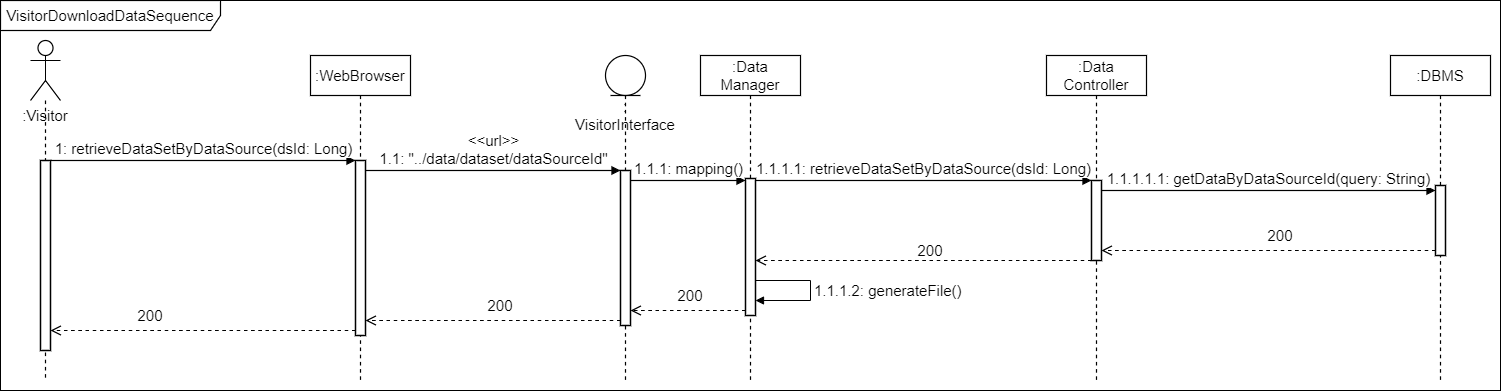
\includegraphics[scale=0.27]{images/runtime_view/visitor_download_data_runtime_view_diagram.png}
        \caption{Visitor downloads data sequence diagram}
        \label{fig:visitor_downloads_data_sequence_diagram}
\end{figure}
\FloatBarrier

Everyone using the platform can also download data sets of interest.\\ 
Clicking the "Download" button associated to the data set of interest the Web Browser will send the request to the DataManager through the VisitorInterface doing a GET to "../data/dataset/\{dataSourceId\}" (where dataSourceId is the id of the dataSource from which the data to be downloaded will be retrieved).
The DataManager calls the DataController to query the DBMS asking for the data set indicated. Once the DataManager is provided with the required data, it generates a file in the selected format and the file is returned to the Visitor with a successful response status code.

\subsubsection{Visitor enters a discussion}

\begin{figure}[h!]
        \centering
        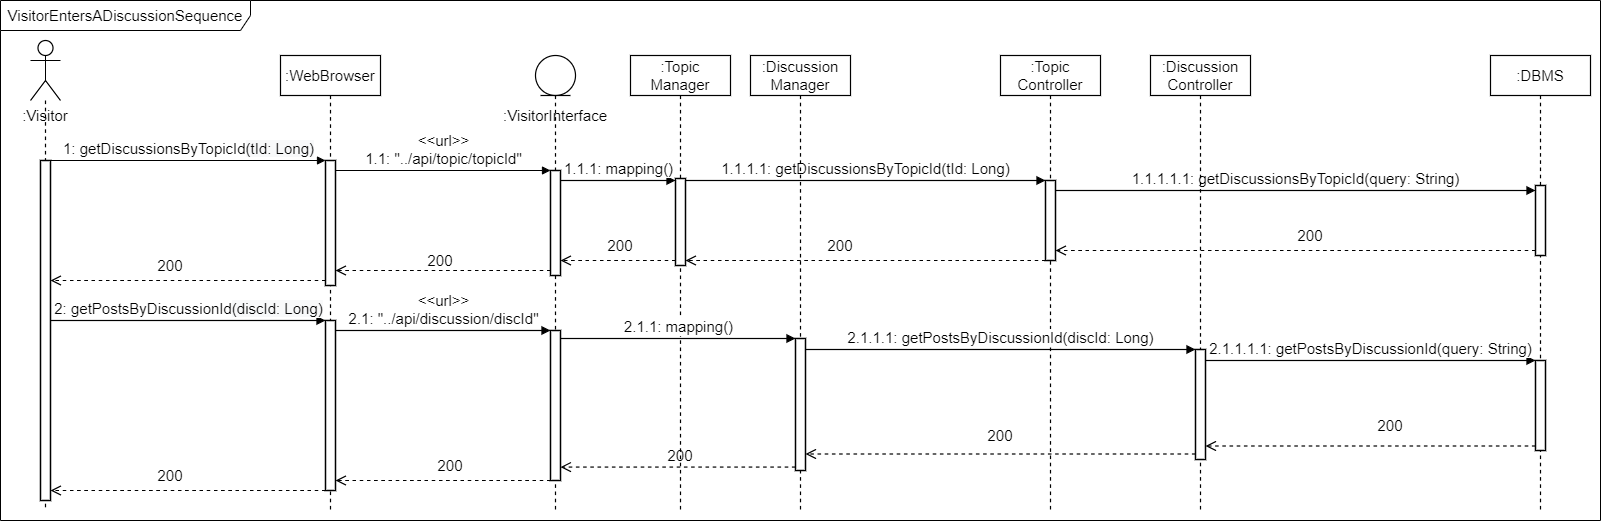
\includegraphics[scale=0.25]{images/runtime_view/visitor_enters_discussion_runtime_view_diagram.png}
        \caption{Visitor enters a discussion sequence diagram}
        \label{fig:visitor_enters_discussion_sequence_diagram}
\end{figure}
\FloatBarrier

In order to consult the forum discussions everyone is able to navigate through the different topics.\\
To do so the first request is send by the Web Browser to the TopicManager via VisitorInterface doing a GET to "../api/topic/\{topicId\}" (where topicId is the id of the topic that contains the discussions the visitor wants to access). The TopicManager will retrieve the list of discussions related to the topic selected from the DBMS using the TopicController. This list will be returned to the Visitor and he will be able to select the one he wants to consult. The Web Browser will forward the request to the DiscussionManager which will call the DiscussionController in order to retrieve from the DBMS the post related to that specific discussion, doing a GET to "../api/discussion/\{discussionId\}".\\
At this point a post list will be returned to the Visitor and a 200 response status code will confirm operation success.

\newpage
\subsubsection{Sign Up}

\begin{figure}[h!]
        \centering
        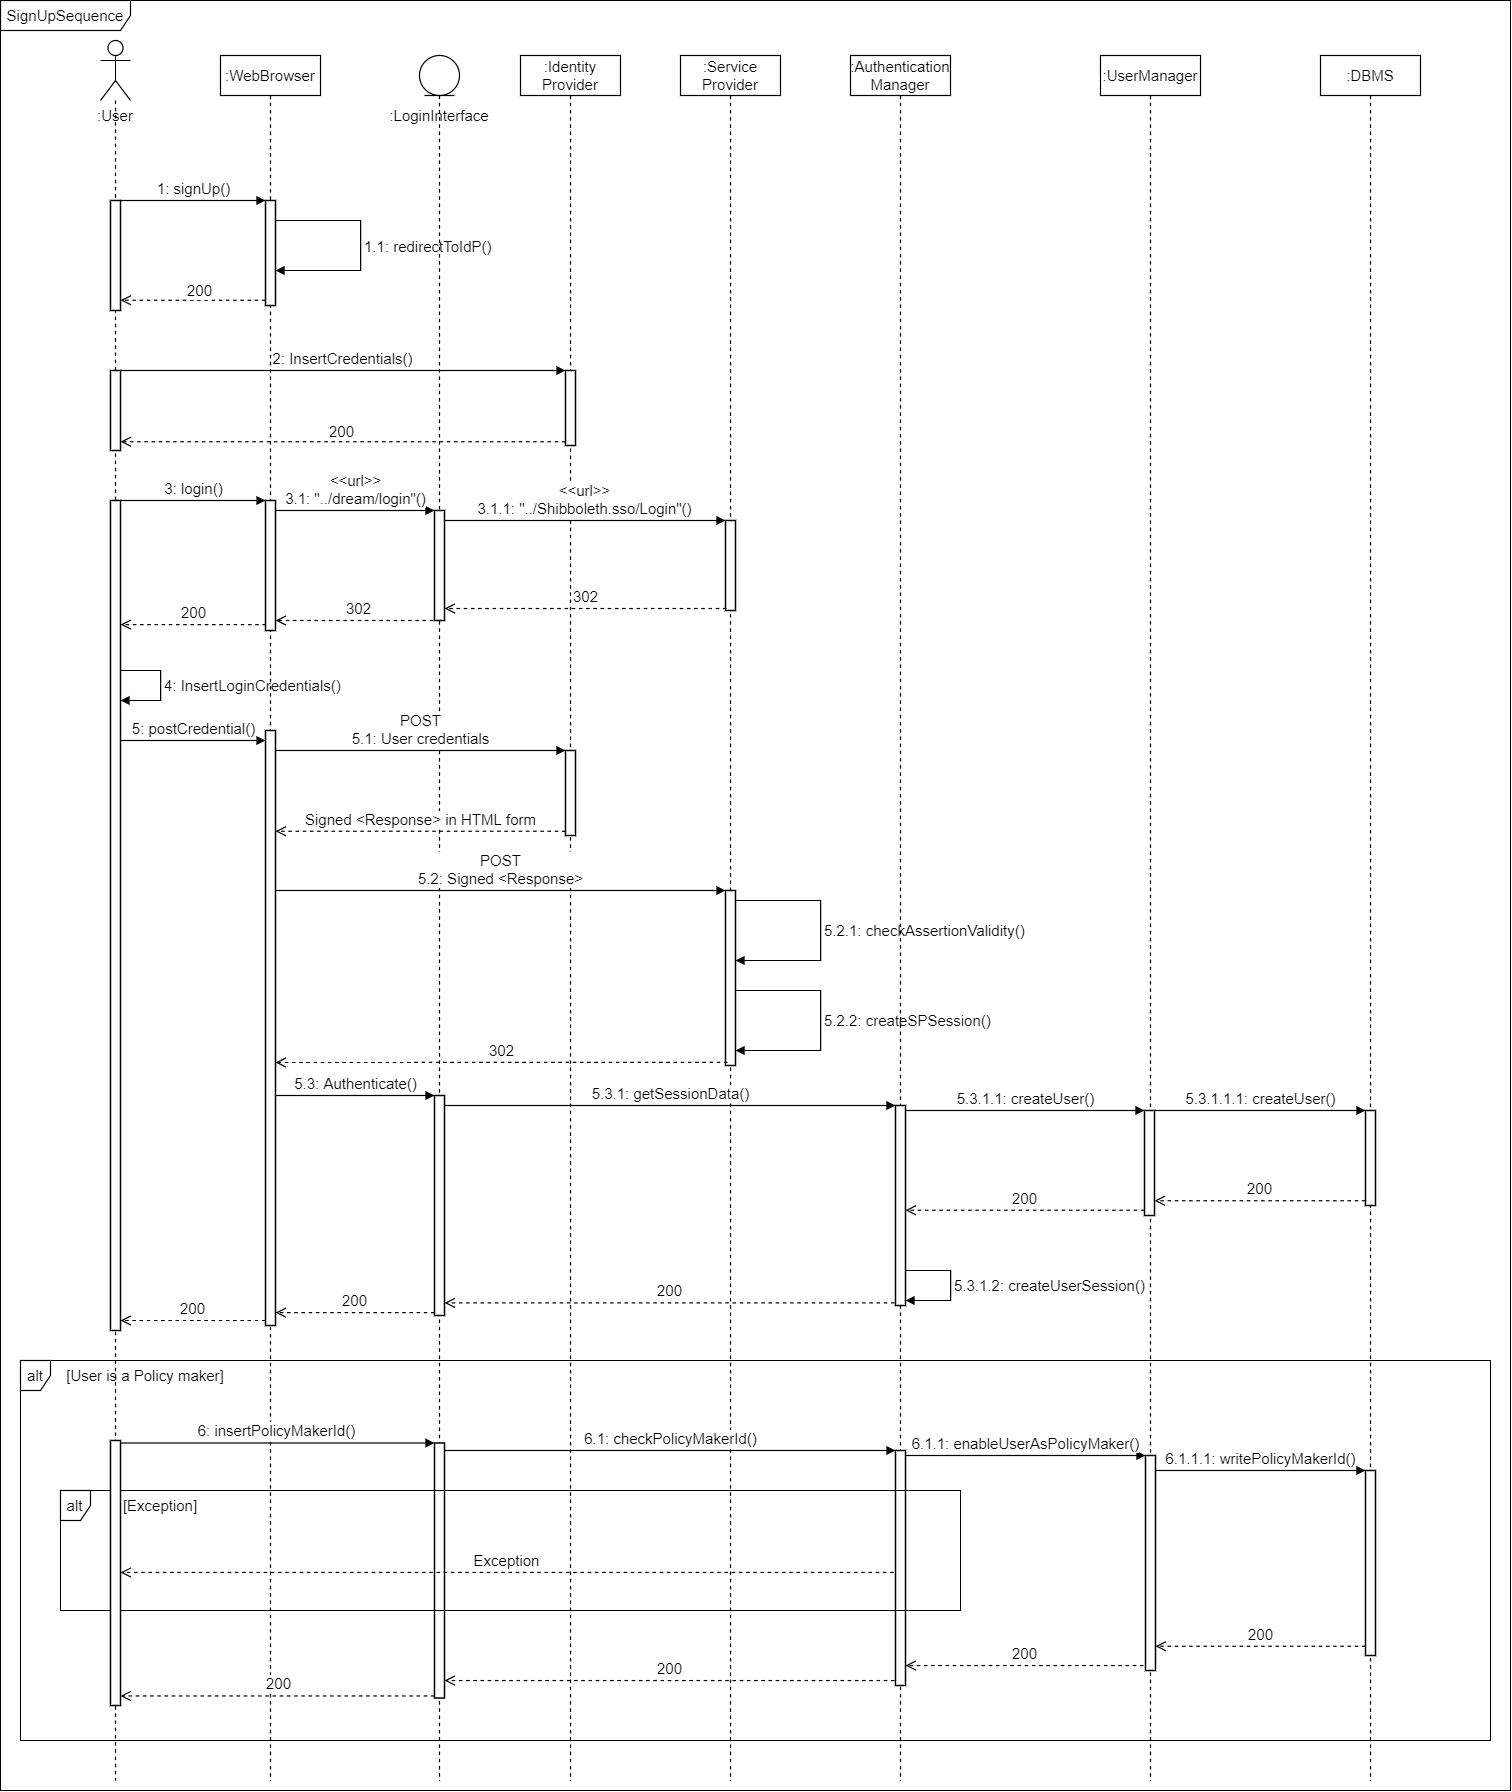
\includegraphics[scale=0.23]{images/runtime_view/signup_runtime_view_diagram.png}
        \caption{Sign Up sequence diagram}
        \label{fig:sign_up_sequence_diagram}
\end{figure}
\FloatBarrier
In order to Sign Up a User is redirect by the Web Browser to the default Identity Provider where he can register his account. When the account creation is completed the User can start again by login. The login action performed by the user is translated in a url ("../dream/login") which is redirected to the Service Provider login initiator url ("../Shibboleth.sso/Login") by the LoginInterface. Now the user is redirected in the Identity Provider login page with a signed authentication request, from where he can login with the account created before. If the IdP authentication is completed successfully a POST to the Service Provider ACS ("../Shibboleth.sso/SAML2/POST") is performed automatically with a signed assertion (authentication response). The Service Provider checks the validity of the received assertion and saves the user data in the Session and returns a redirect request to the dream single-sign-on page managed by the AuthenticationManager. Now the session data are read, a new user is created by the UserManager and saved in the database by the DBMS. Once the new user is created the AuthenticationManager creates a local user session to complete the login action.
If the received user role is compatible with the Policy maker one, the user is asked to insert a PolicyMakerID to verify the new account, the inserted value is sent to the AuthenticationManager to be verified and, if correct, the UserManager proceeds to update the user in the DBMS with the new role.

\subsubsection{Login}

\begin{figure}[h!]
        \centering
        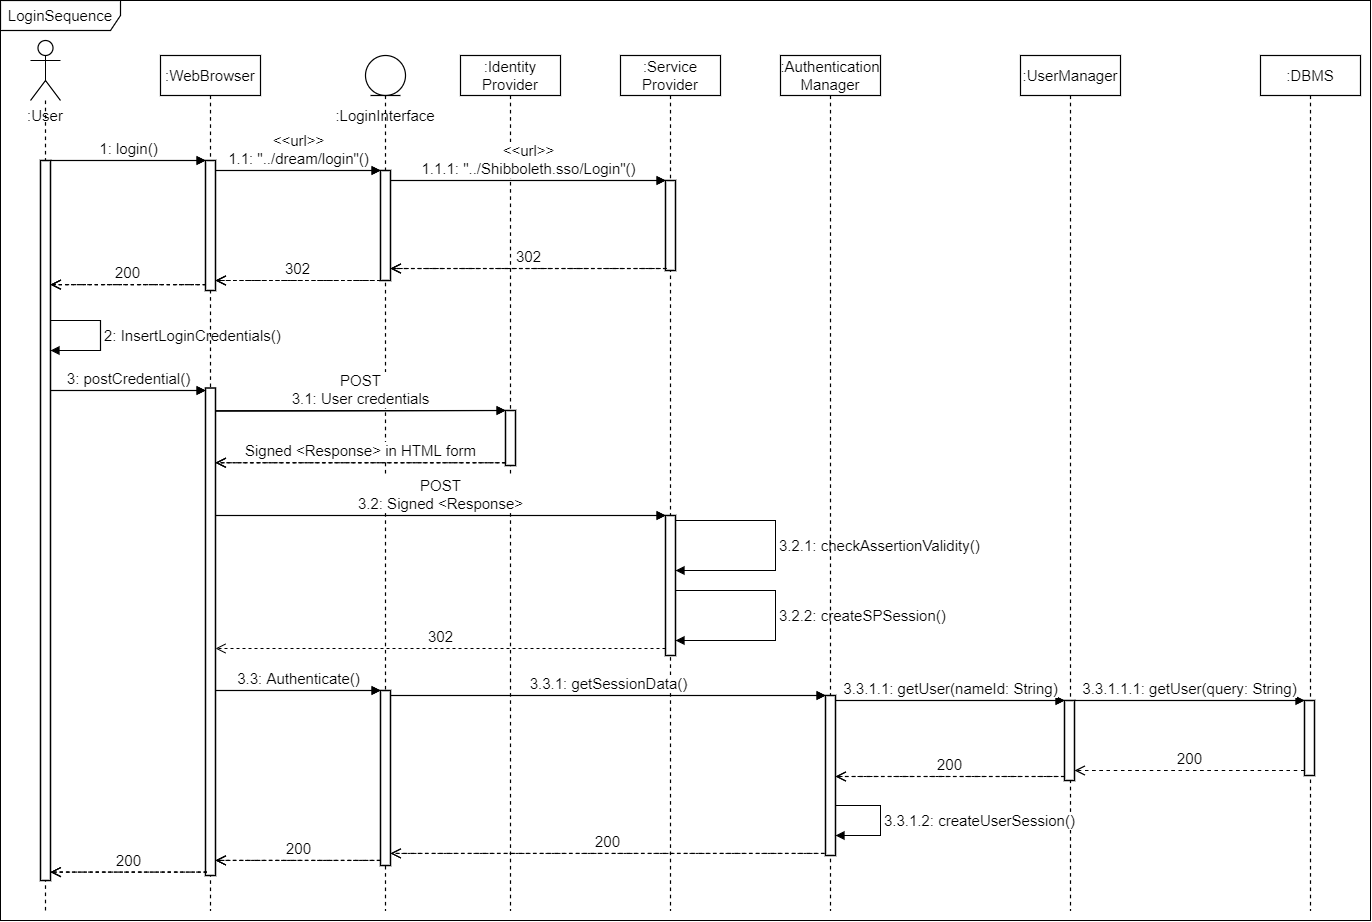
\includegraphics[scale=0.25]{images/runtime_view/login_runtime_view_diagram.png}
        \caption{Login sequence diagram}
        \label{fig:login_sequence_diagram}
\end{figure}
\FloatBarrier
In order to login a User or a Policy Maker the web browser sends a request to the loginInterface ("../dream/login") which will invoke the Service Provider. The provider will return a temporary redirection (http code:302) to the Identity Provider containing a signed authentication request. The Identity Provider will recognize the service request and let the user to authenticate with the IdP credential. After the user is logged in the IdP, it will post the signed assertion (authentication response) to the Service Provider ACS with the user requested data that will be saved in the server session. This will let the AuthenticationManager to create a session retrieving the data from the DBMS passing through the UserManager's getUser() request. At the end a 200 response status code will be sent to the User.

\subsubsection{Login Administrator}

\begin{figure}[h!]
        \centering
        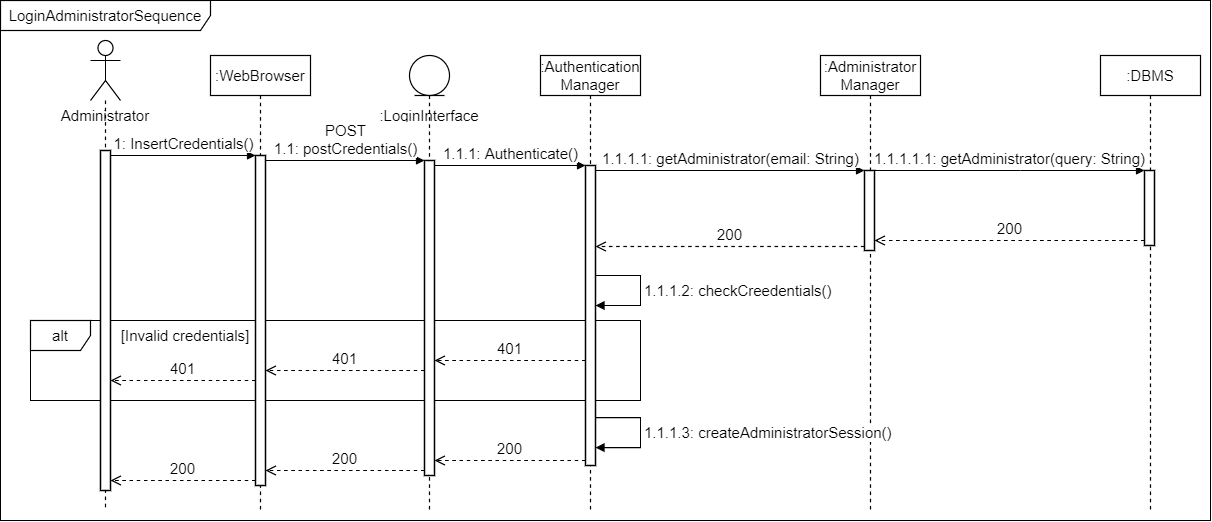
\includegraphics[scale=0.30]{images/runtime_view/login_administrator_runtime_view_diagram.png}
        \caption{Login Administrator sequence diagram}
        \label{fig:login_administrator_sequence_diagram}
\end{figure}
\FloatBarrier

The Administrator login process works differently because it doesn't relies on an external services.\\
First of all, the Administrator will insert the login credentials and those will be sent to the LoginInterface. The AuthenticationManager invoked by the interface will retrieve the Administrator data from the DBMS calling the AdministratorManager. AuthenticationManager at this point checks the credentials: if they are invalid it will respond with a 401 (unauthorized) http status code, otherwise an Administrator session will be created and a 200 response status code will be sent to the Administrator.

\newpage
\subsubsection{Publish a post by User}

\begin{figure}[h!]
        \centering
        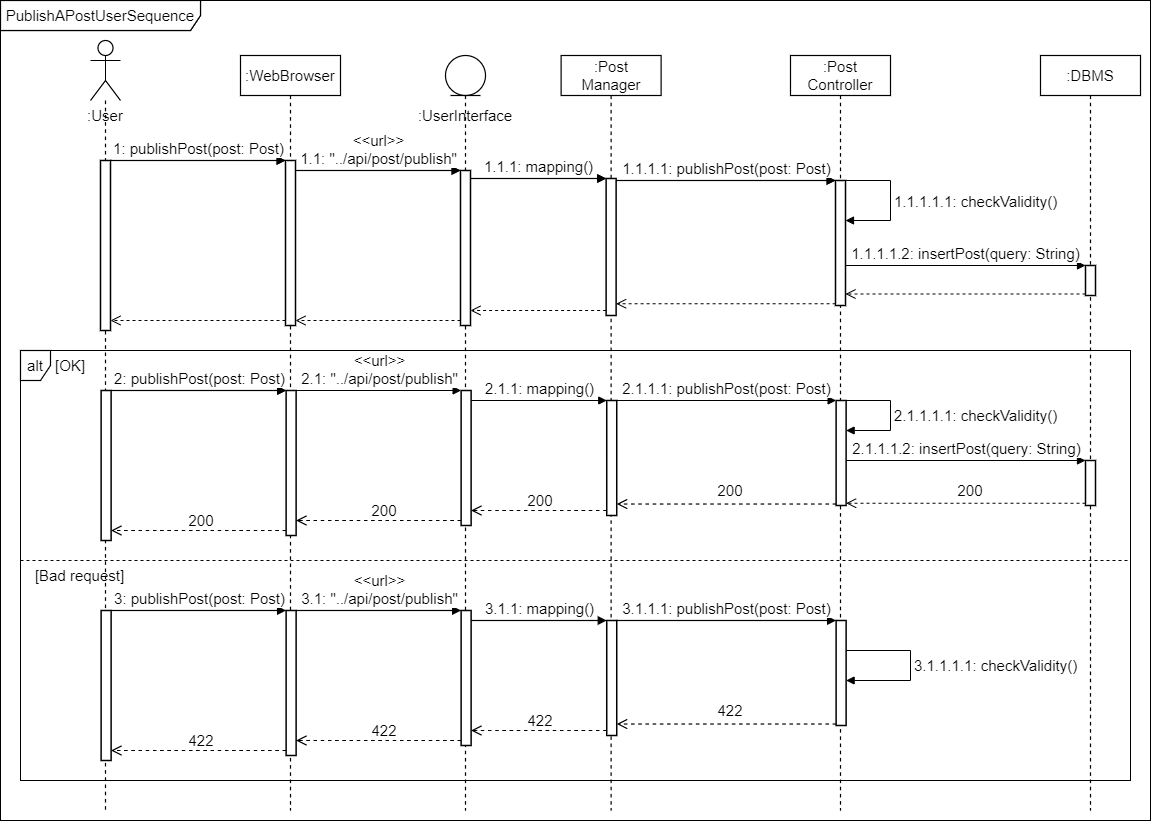
\includegraphics[scale=0.30]{images/runtime_view/publish_post_user_runtime_view_diagram.png}
        \caption{Publish a post by User sequence diagram}
        \label{fig:publish_a_post_by_user_sequence_diagram}
\end{figure}
\FloatBarrier

After writing the post, the User tries to publish it by clicking on publish a post in the Web Browser. This will contact the PostManager via UserInterface doing a POST to "../api/post/publish".\\
The PostManager then calls the PostController which sends an insert query to the DBMS. The post will be added to the post table with pending status, waiting for Policy maker approval.

\newpage
\subsubsection{Publish a post by Policy Maker}

\begin{figure}[h!]
        \centering
        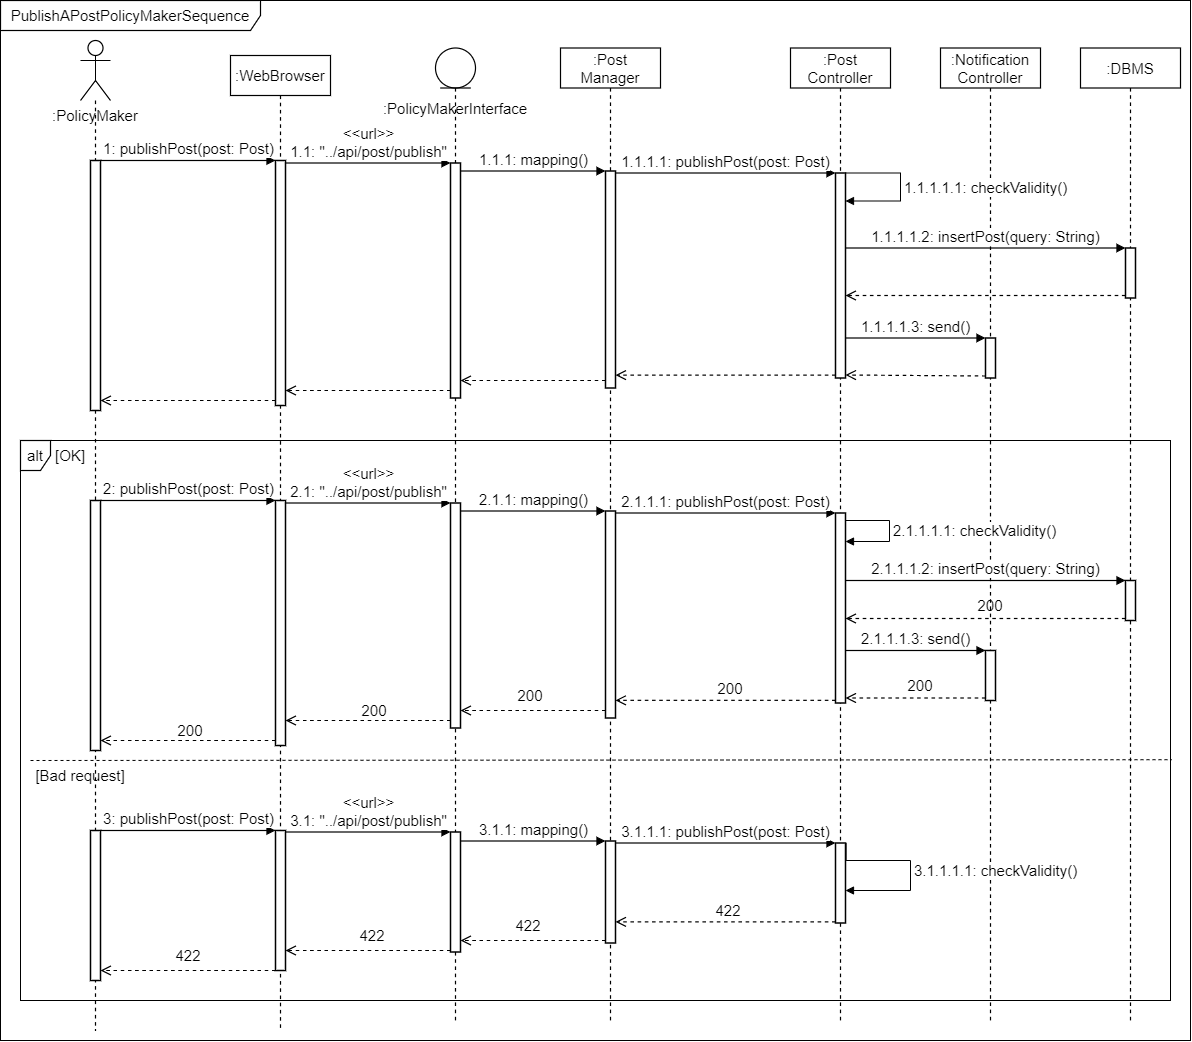
\includegraphics[scale=0.30]{images/runtime_view/publish_post_policy_maker_runtime_view_diagram.png}
        \caption{Publish a post by Policy Maker sequence diagram}
        \label{fig:publish_a_post_policy_maker_sequence_diagram}
\end{figure}
\FloatBarrier

It is a very similar process to the one ran by the User but it has some relevant differences.\\
When a Policy maker tries to publish a post, the PolicyMakerInterface, invoked by the Web Browser doing a POST to "../api/post/publish", contacts the PostManager which inserts the post in the DBMS via the PostController. In this case the post is immediately available from the forum and doesn't need for approval. The PostController will then invoke the NotificationController in order to send a notification to the list of users that follow the discussion.

\newpage
\subsubsection{Modify a post}

\begin{figure}[h!]
        \centering
        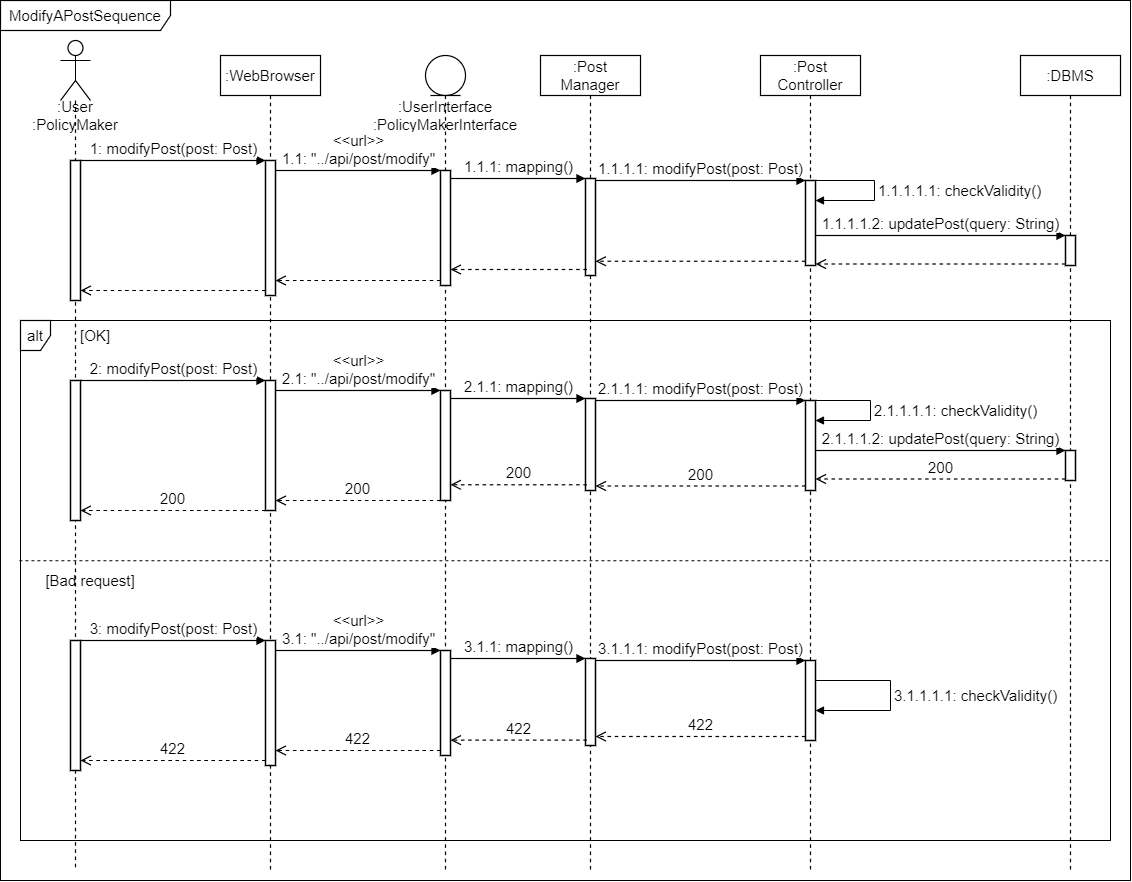
\includegraphics[scale=0.30]{images/runtime_view/modify_post_runtime_view_diagram.png}
        \caption{Modify a post sequence diagram}
        \label{fig:modify_a_post_sequence_diagram}
\end{figure}
\FloatBarrier

When a User or a Policy maker wants to modify a post, after making the desired changes, the PostManager is invoked by the Web Browser via the PolicyMakerInterface doing a POST to "../api/post/modify". \\
The PostManager then calls the PostController which queries for an update in the indicated post. If the operation is successful, a 200 response status code is returned to the User/Policy maker.

\newpage
\subsubsection{Delete a post}

\begin{figure}[h!]
        \centering
        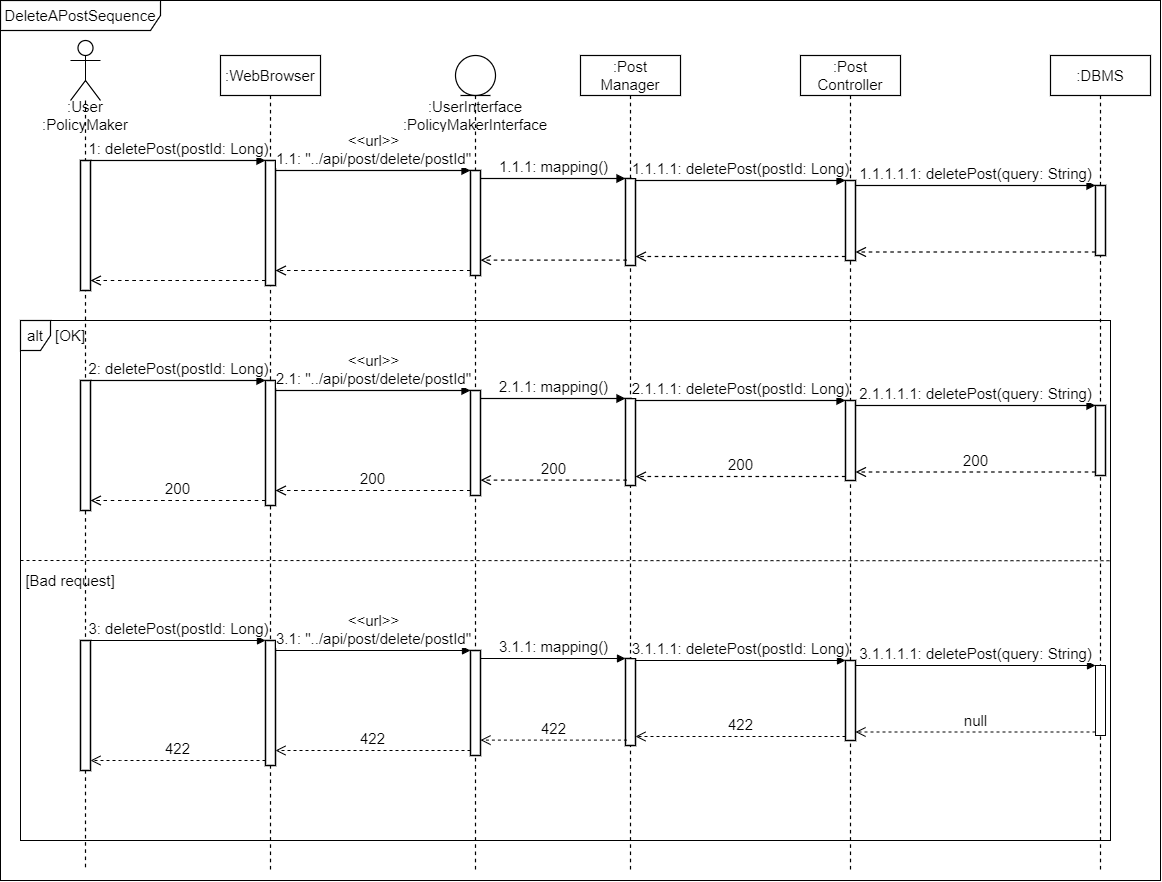
\includegraphics[scale=0.30]{images/runtime_view/delete_post_runtime_view_diagram.png}
        \caption{Delete a post sequence diagram}
        \label{fig:delete_a_post_sequence_diagram}
\end{figure}
\FloatBarrier

When a User or a Policy maker wants to delete a post, the PostManager is invoked by the Web Browser via the PolicyMakerInterface doing a POST to "../api/post/delete/\{postId\}" (where postId is the id of the post to be deleted). \\
The PostManager then calls the PostController which queries for a delete of the post. If the operation is successful, a 200 response status code is returned to the User/Policy maker.

\newpage
\subsubsection{Create a discussion}

\begin{figure}[h!]
        \centering
        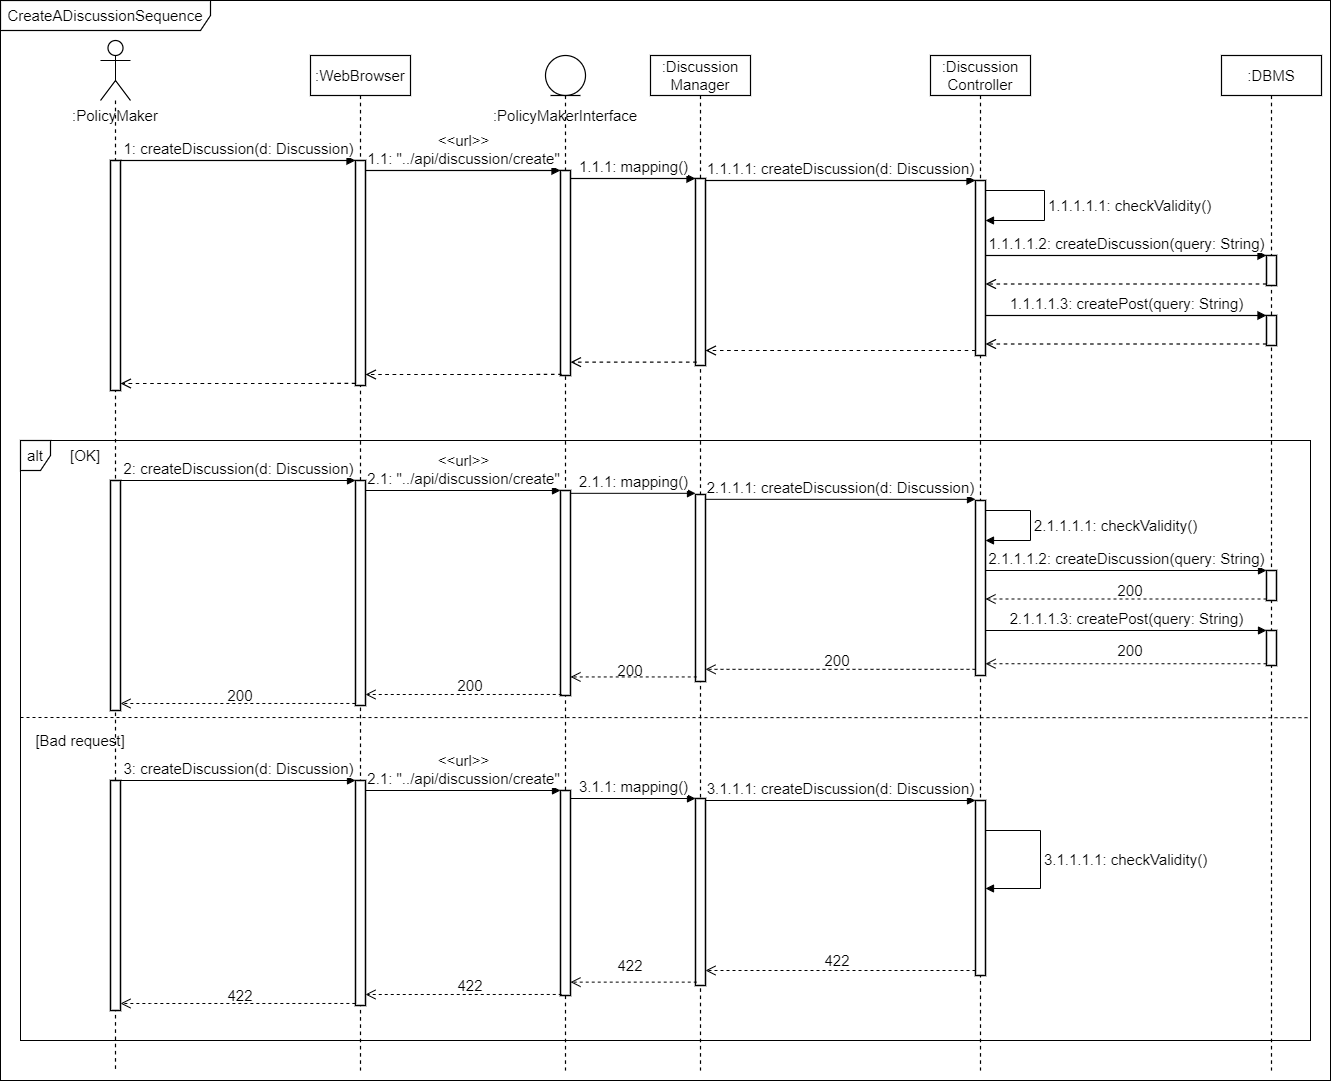
\includegraphics[scale=0.27]{images/runtime_view/create_discussion_runtime_view_diagram.png}
        \caption{Create a discussion sequence diagram}
        \label{fig:create_a_discussion_sequence_diagram}
\end{figure}
\FloatBarrier

A Policy maker, in order to create a discussion, will use the "create a discussion" button that will call the PolicyMakerInterface doing a POST to "../api/discussion/create". The request will be forwarded to the DiscussionManager, which will query the DBMS via the DiscussionController in order to insert a new discussion. Every discussion requires at least one post, so when the DBMS will insert the new discussion the DiscussionController will ask the DBMS to insert the post passed into the Discussion object. A 200 response status code will inform the Policy maker that the operation was successful.

\newpage
\subsubsection{Delete a discussion}

\begin{figure}[h!]
        \centering
        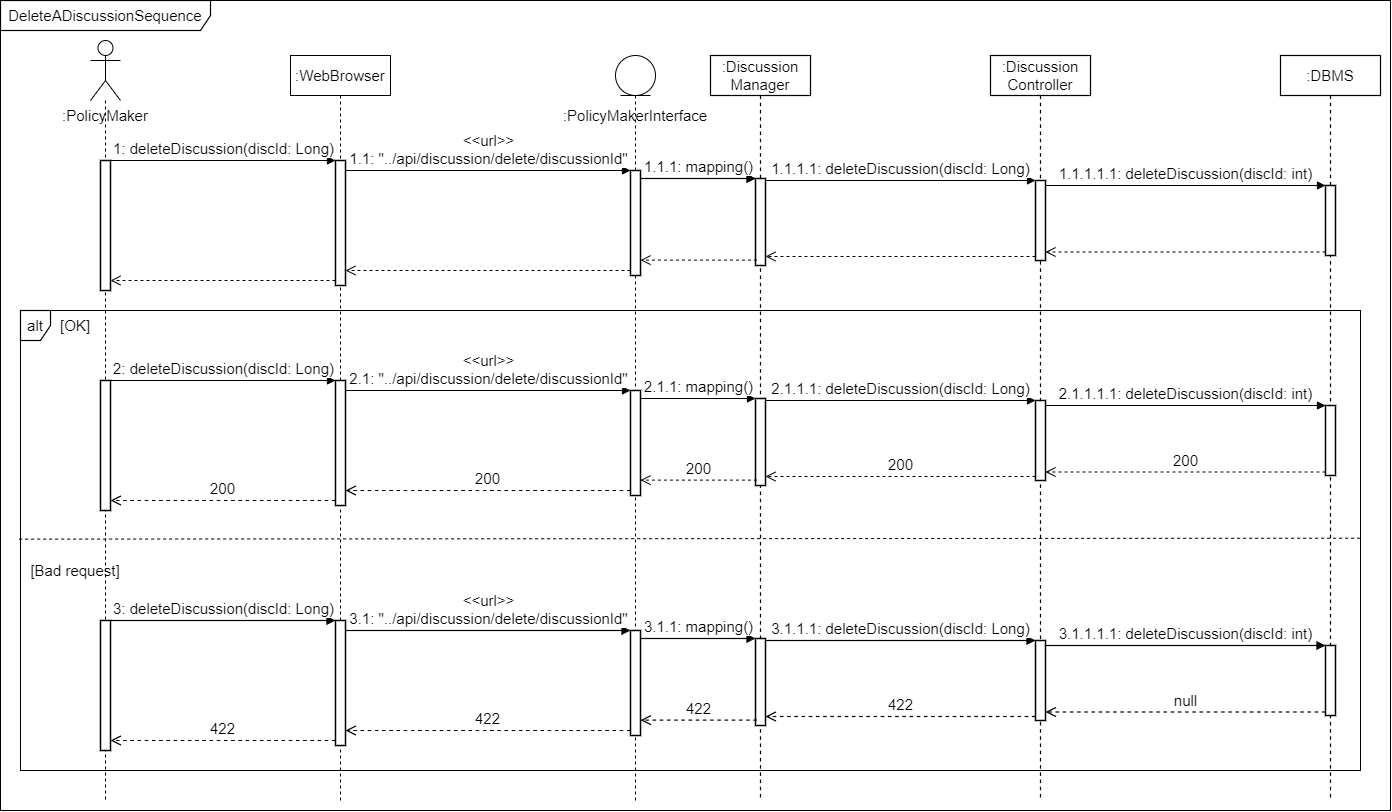
\includegraphics[scale=0.25]{images/runtime_view/delete_discussion_runtime_view_diagram.png}
        \caption{Delete a discussion sequence diagram}
        \label{fig:delete_a_discussion_sequence_diagram}
\end{figure}
\FloatBarrier

In order to remove a whole discussion from the forum, a Policy maker will invoke the PolicyMakerInterface via Web Browser doing a POST to "../api/discussion/delete/\{discussionId\}" (where discussionId is the id of the discussion to be deleted). The request will be forwarded to the DiscussionManager, which will call the DiscussionController in order to remove the discussion and the relative posts from the DBMS. A 200 response status code will inform the Policy Maker that the operation was successful.

\subsubsection{Confirm pending post}

\begin{figure}[h!]
        \centering
        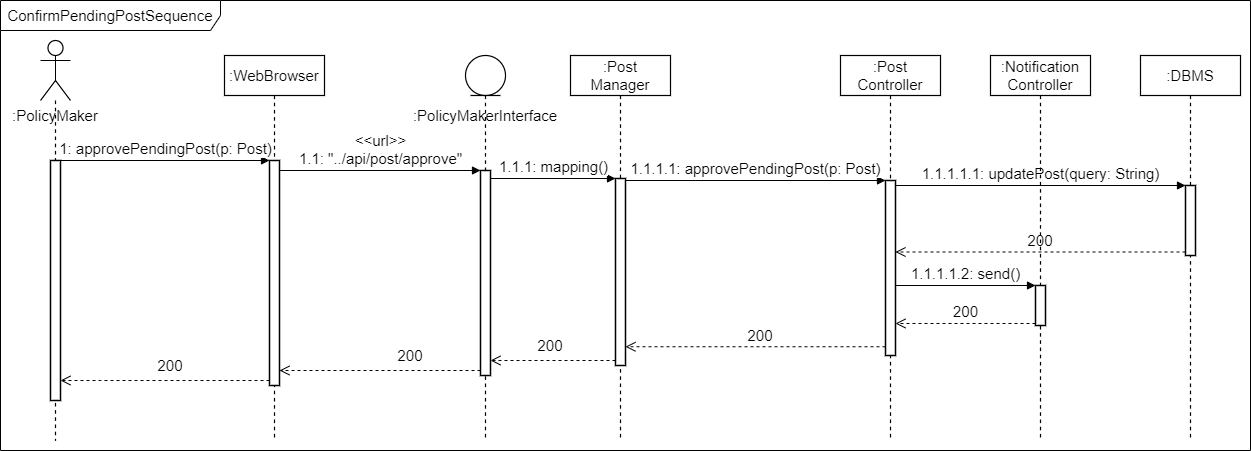
\includegraphics[scale=0.25]{images/runtime_view/confirm_pending_post_runtime_view_diagram.png}
        \caption{Confirm a pending post sequence diagram}
        \label{fig:confirm_pending_post_sequence_diagram}
\end{figure}
\FloatBarrier

Before a post written by a User is visible in the forum, it is necessary that the Policy maker approves its publication.\\ 
To do so, a Policy maker will click on "Approve pending post" button and the Web Browser will call the PolicyMakerInterface doing a POST to "../api/post/approve". The request will be forwarded to the PostManager and the PostController will be invoked to update the post's status field. Then, the PostController will call the NotificationController in order to notify its publication in the forum to the creator of the post and to the other users following the discussion in which that post is being published. A 200 response status code will inform the Policy maker that the operation was successful.

\subsubsection{Decline pending post}
\begin{figure}[h!]
        \centering
        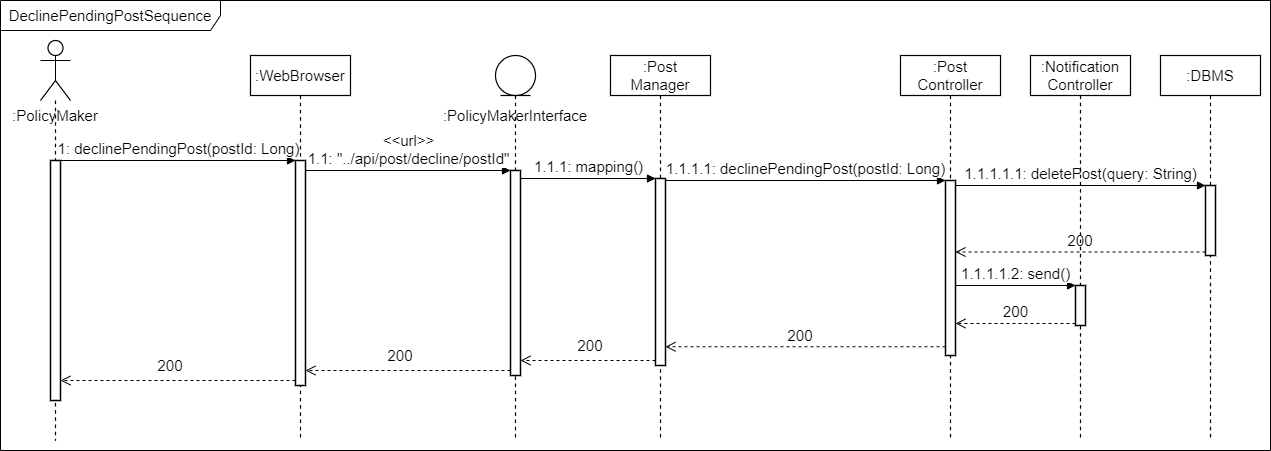
\includegraphics[scale=0.27]{images/runtime_view/decline_pending_post_runtime_view_diagram.png}
        \caption{Decline a pending post sequence diagram}
        \label{fig:decline_pending_post_sequence_diagram}
\end{figure}
\FloatBarrier

Some posts should not be made public because they do not follow the forum rules or are not related to the discussion topics.\\ 
To do so, a Policy maker will click on "Decline pending post" button and the Web Browser will call the PolicyMakerInterface doing a POST to "../api/post/decline/\{postId\}" (where postId is the id of the post to be declined). The request will be forwarded to the PostManager and the PostController will be deleted from the DataBase. Then, the PostController will call the NotificationController in order to warn the creator that his post will not be published in the forum. A 200 response status code will inform the Policy Maker that the operation was successful.

\newpage
\subsubsection{Recalculate new Deviance}

\begin{figure}[h!]
        \centering
        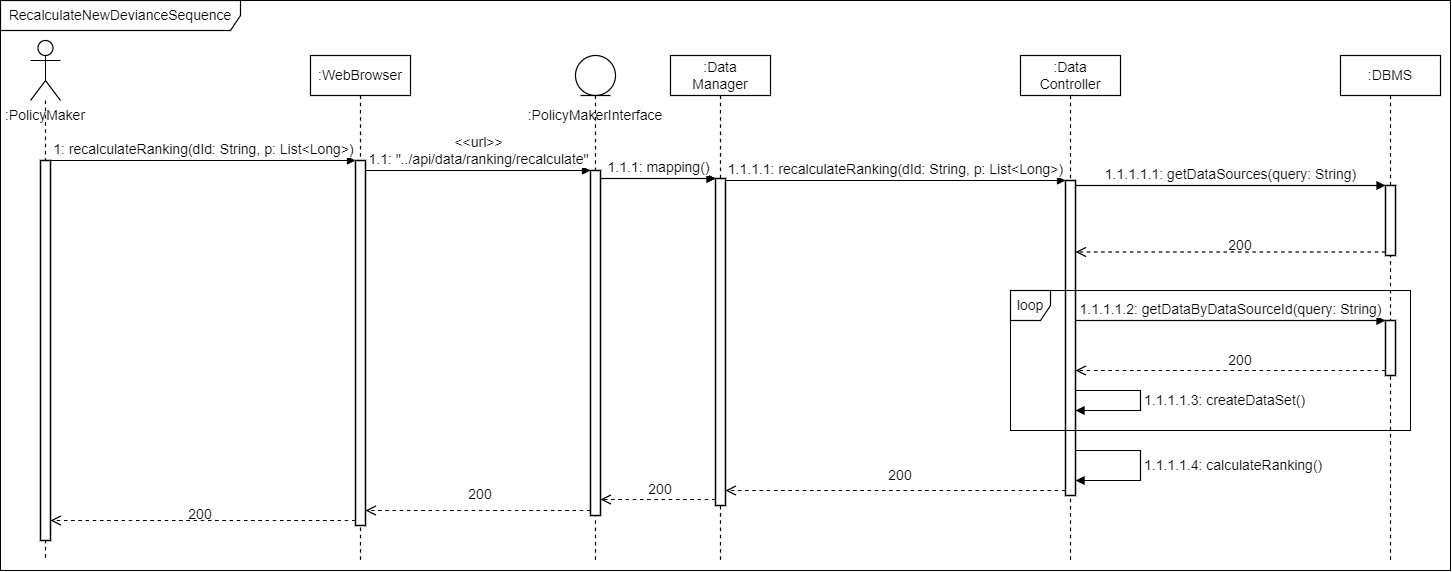
\includegraphics[scale=0.27]{images/runtime_view/recalculate_new_deviance_runtime_view_diagram.png}
        \caption{Recalculate new Deviance sequence diagram}
        \label{fig:deviance_recalculate_sequence_diagram}
\end{figure}
\FloatBarrier

A Policy maker might want to recalculate the Deviance using a different set of parameters than the standard one.\\
To do this, once he has selected all the parameters of his interest, the Policy maker will call the "recalculateRanking" function and the Web Browser will forward his request to the PolicyMakerInterface doing a GET to "../api/data/ranking/recalculate". This request is submitted to the DataManager which queries the DBMS via the DataController. Using the data retrieved, the DataController enters in a loop in which retrieves all the data of a single data source and for that data it creates a dataSet. After creating all the datasets, the DataController use the algorithm to create a ranking using all the different data sets just built. In the end, the result of the ranking algorithm are sent back to the Policy maker.

\newpage
\subsubsection{Add a new data source}

\begin{figure}[h!]
        \centering
        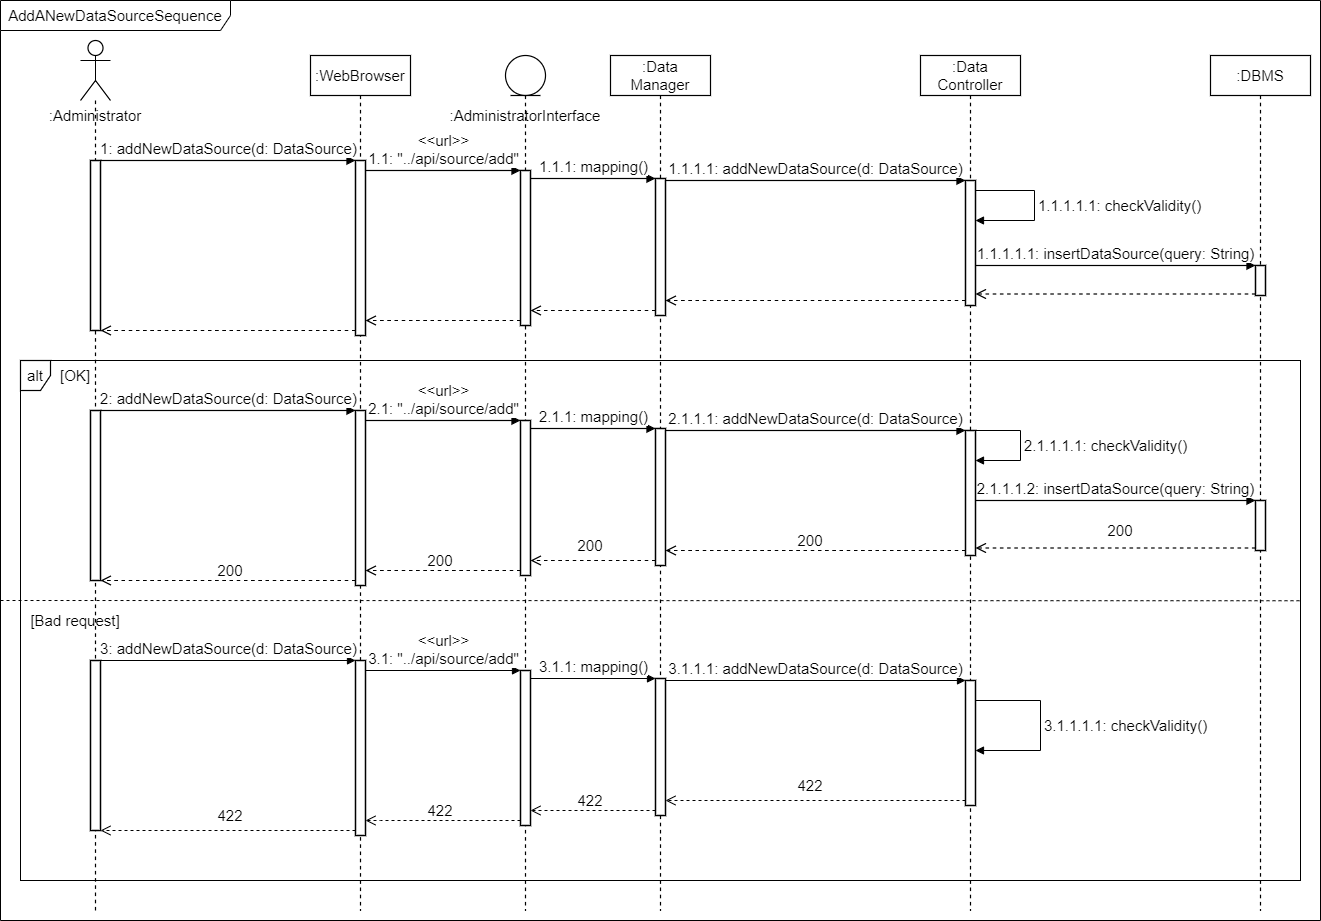
\includegraphics[scale=0.27]{images/runtime_view/add_new_data_source_runtime_view_diagram.png}
        \caption{Add a new data source sequence diagram}
        \label{fig:add_new_data_source_sequence_diagram}
\end{figure}
\FloatBarrier

To add a new data source, an Administrator will have to invoke the "addNewDataSource()" method.\\
This will call the AdministratorInterface via Web Browser by doing a POST to "../api/source/add". The interface calls the DataManager which will insert the data source in the DBMS via DataController. 
A 200 response code status delivered to the Administrator will let him know that the operation was successful, otherwise a 422 response status code will tell that the request wasn't able to be processed.

\newpage
\subsubsection{Modify a data source}

\begin{figure}[h!]
        \centering
        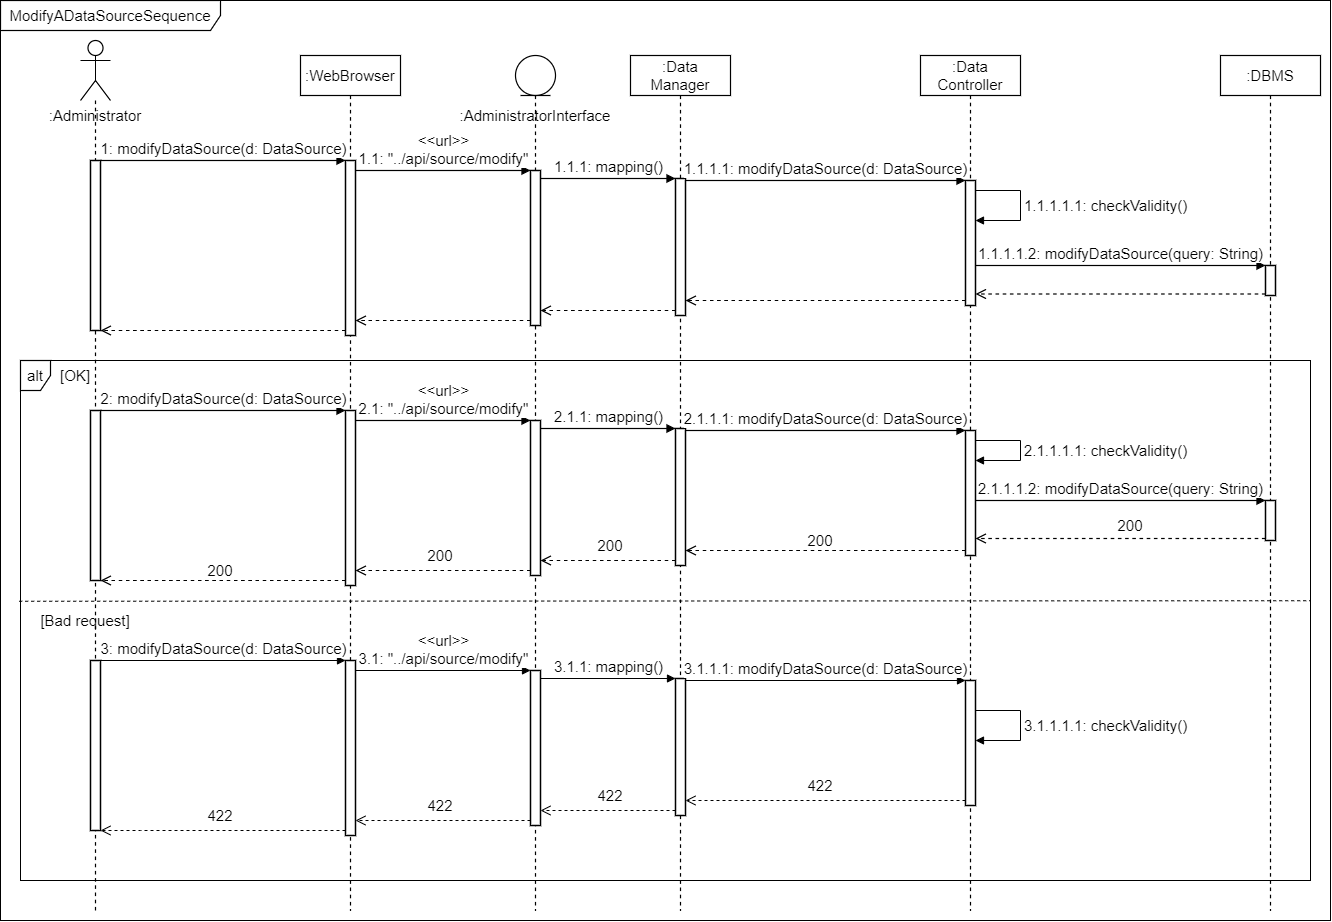
\includegraphics[scale=0.27]{images/runtime_view/modify_data_source_runtime_view_diagram.png}
        \caption{Modify a data source sequence diagram}
        \label{fig:modify_data_source_sequence_diagram}
\end{figure}
\FloatBarrier

In order to modify a data source an Administrator invoke the AdministratorInterface via Web Browser by doing a POST to "../api/source/modify". The data are sent to the DataManager which will update the DBMS record calling the DataController.
A 200 response code status delivered to the Administrator will let him know that the operation was successful, otherwise a 422 response status code will tell that the request wasn't able to be processed.

\newpage
\subsubsection{Remove a data source}

\begin{figure}[h!]
        \centering
        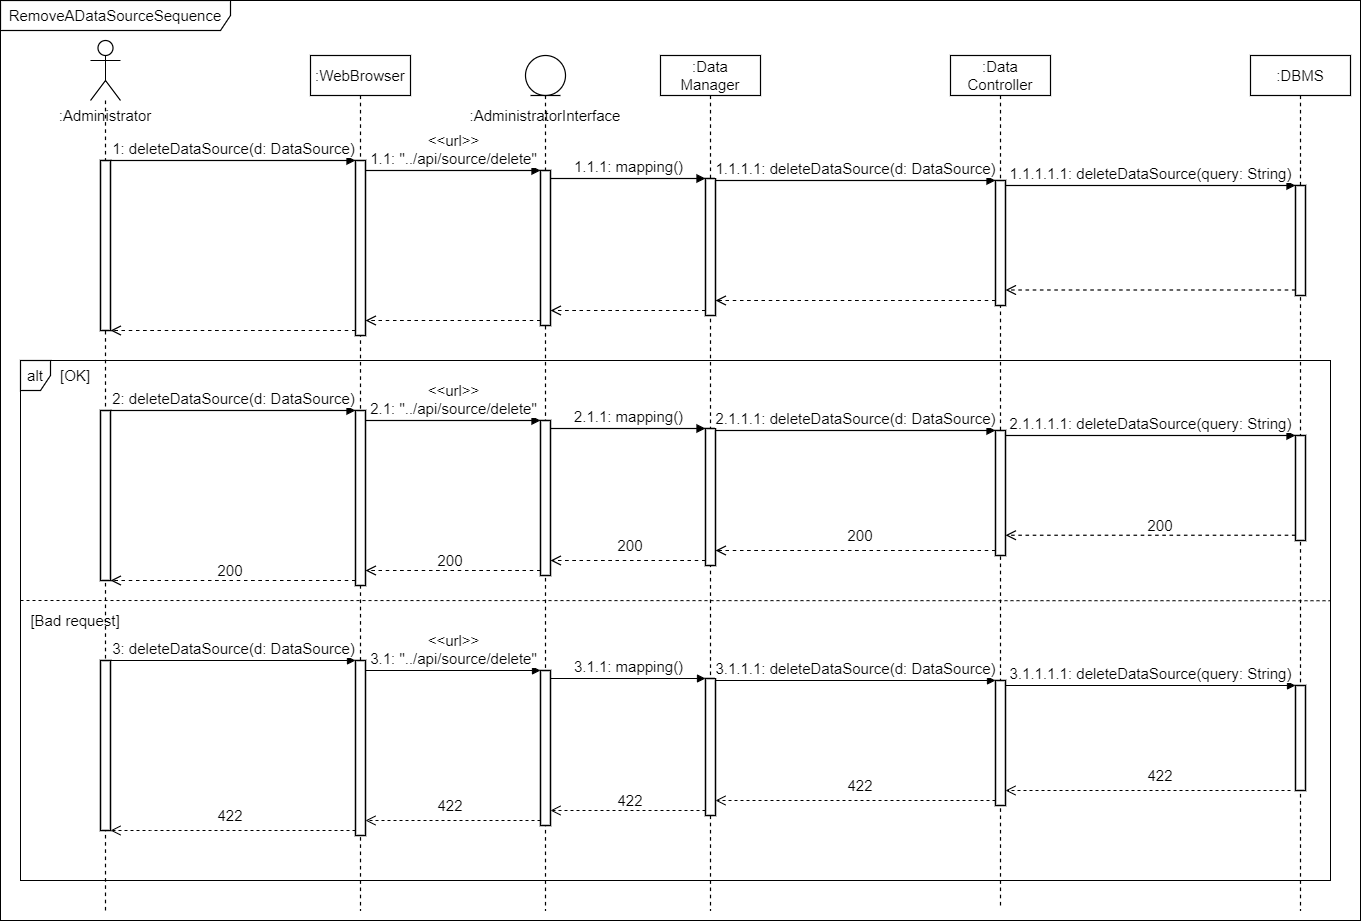
\includegraphics[scale=0.27]{images/runtime_view/remove_data_source_runtime_view_diagram.png}
        \caption{Remove a data source sequence diagram}
        \label{fig:remove_data_source_sequence_diagram}
\end{figure}
\FloatBarrier

An obsolete data source can be removed by an Administrator. \\
To do so the AdministratorInterface is invoked via Web Browser by doing a POST to "../api/source/delete/{sourceId}" (where sourceId is the id of the source to be deleted). The interface calls the DataManager which will remove the data source from the DBMS via DataController. 
A 200 response code status delivered to the Administrator will let him know that the operation was successful, otherwise a 422 response status code will tell that the request wasn't able to be processed.

\newpage
\subsection{Component Interfaces}

\begin{figure}[h!]
        \centering
        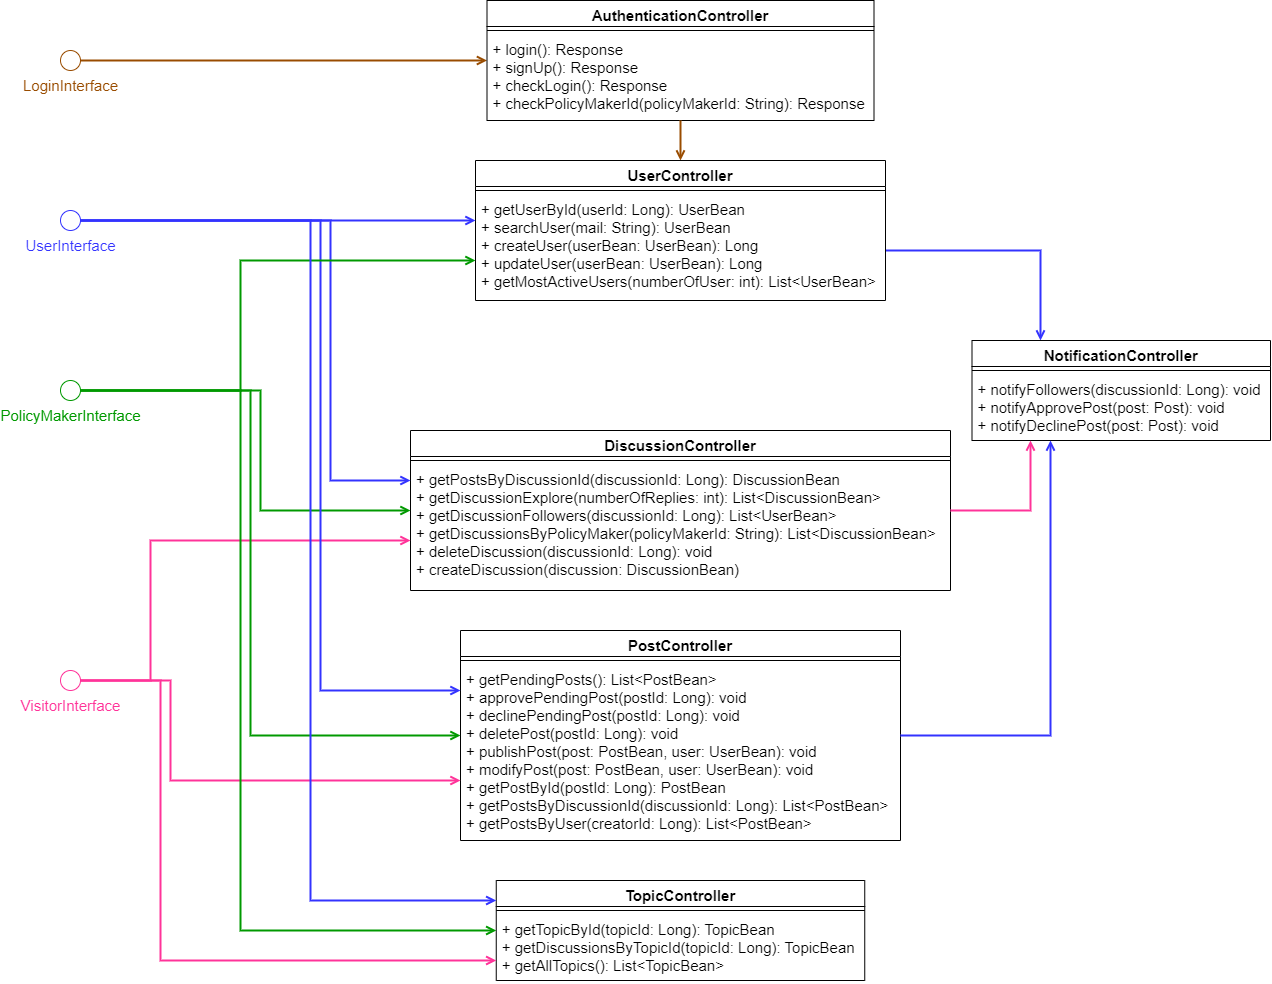
\includegraphics[scale=0.34]{images/component_interfaces/forum_component_interface.png}
        \caption{Forum Interfaces Diagram}
        \label{fig:forum_interfaces_diagram}
\end{figure}
\FloatBarrier

In figure \ref{fig:forum_interfaces_diagram} the principal interfaces to make Dream Forum run are shown.\\
Starting from the beginning the LoginInterface is needed to make the login and the sign up possible. It is realized through the AuthenticationController which is also used by the UserController to check permissions in the operations.\\
The UserInterface provides all the functionalities needed by a User such as the management of his account, the possibility to retrieve his own replies and to create, modify and delete a post. These functionalities are implemented by four controllers: the UserController and the different controllers of the forum: TopicController, DiscussionController and PostController.\\
The PolicyMakerInterface is quite similar to the User one but provides additional methods for the forum moderation such as the creation of a discussion or the possibility to modify/delete other User's posts. These functionalities are implemented by four controllers: the UserController and the different controllers of the forum: TopicController, DiscussionController and PostController.\\
The NotificationController is used by the UserController, the DiscussionController and the PostController to send email notification when needed and, finally, the VisitorInterface relies on the different controllers of the forum: TopicController, DiscussionController and PostController.

\begin{figure}[h!]
        \centering
        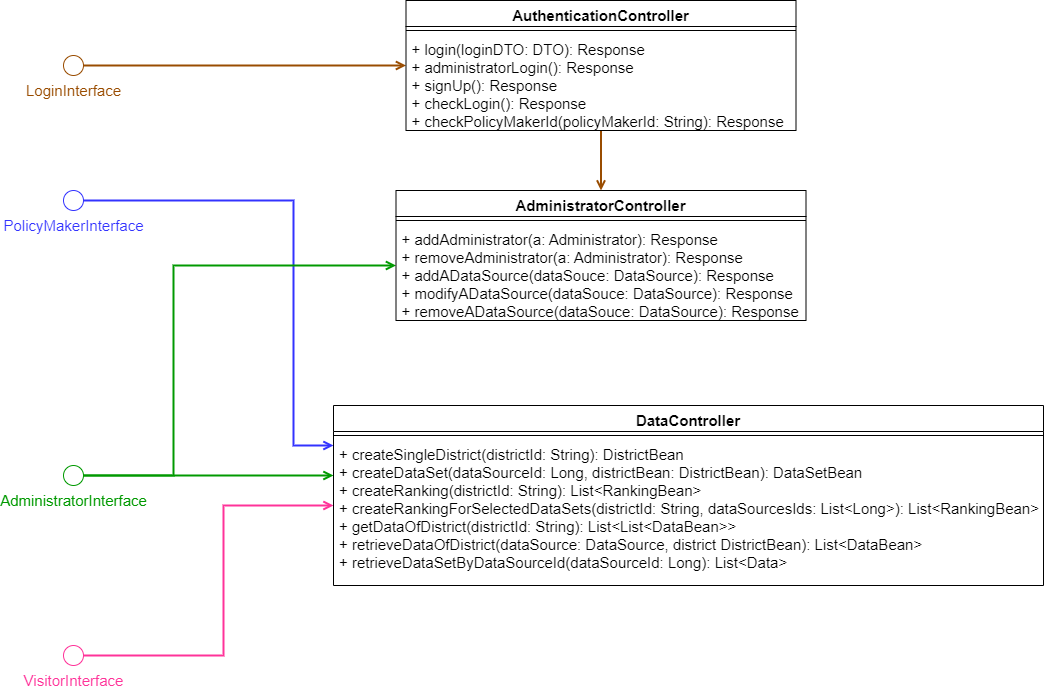
\includegraphics[scale=0.38]{images/component_interfaces/data_component_interface.png}
        \caption{Data Interfaces Diagram}
        \label{fig:data_interfaces_diagram}
\end{figure}
\FloatBarrier

In figure \ref{fig:data_interfaces_diagram} the principal interfaces to make Dream Data aggregator run are shown.\\
Starting from the beginning, the LoginInterface is required to let Administrators (local authentication) and Policy makers (IdP authentication) to login. It uses the AuthenticationController which provides both the function for the Administrators authentication and the external one.\\
The PolicyMakerInterface provides all the functionalities used by a Policy maker such as using the deviance algorithm and have access to the data, that are handled by the DataController.\\
The AdministratorInterface, instead, provides the admin functionalities like adding or remove a new administrator by means of the AdministratorController and add, modify and remove data-sources with the help of the DataController.\\
Finally, the VisitorInterface relies on the DataController which let the visitors to retrieve all the public content they can access to.
\newpage

\subsection{Logical Description of Data}

\begin{figure}[h!]
        \centering
        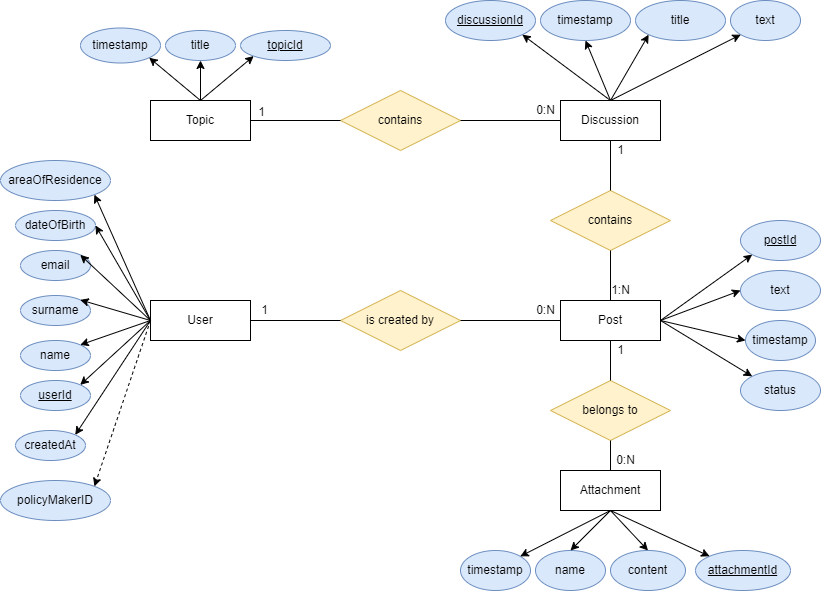
\includegraphics[scale=0.35]{images/er_diagrams/forum_er_diagram.png}
        \caption{Forum ER Diagram}
        \label{fig:forum_er_diagram}
\end{figure}
\FloatBarrier

\begin{figure}[h!]
        \centering
        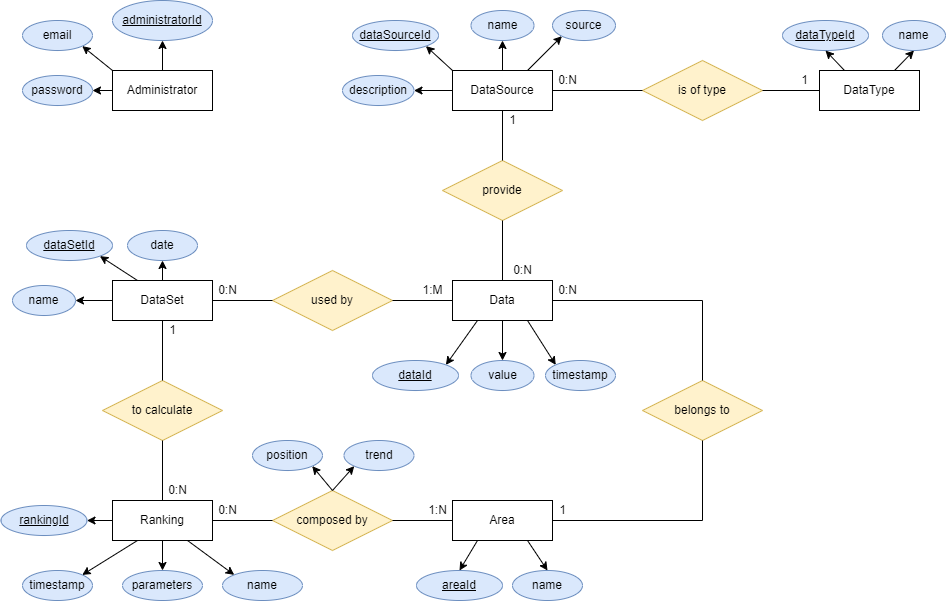
\includegraphics[scale=0.35]{images/er_diagrams/data_er_diagram.png}
        \caption{Data ER Diagram}
        \label{fig:data_er_diagram}
\end{figure}
\FloatBarrier

The two figures above show the database structure for the forum and the data sections.\\
In the first one the hierarchical structure of the forum (fig: \ref{fig:forum_er_diagram}) is evident thanks to the division in topic, discussion and post. The topic category may not contain any discussion in a first moment, but the discussion category needs to always have at least one post related. A post is connected also to his creator, which can be either a User or a Policy maker. The Policy maker differs from the User because it is identified with a non-null value in the policyMakerID field.
The post table is also connected to the attachment one: a post can have more than one attachment.\\

The Data ER diagram (fig: \ref{fig:data_er_diagram}) shows how the different information that concern the data that Dream platform provides needs to be organized. An administrator table will be necessary to store the Administrator login credentials because they don't rely over the external provider.
The data source will be linked to the data it provides and in the DataType table will be presented the data type related to the data supplied. The adoption of a table instead of using a simple enumeration consents to dynamically change the data type presents in the database. Data will be linked to the Area of their competence.
A Data set will be established by different data and those data could be used by different data set. This is why a bridge table will be needed to link the two tables. Each data set will be used to calculate different ranking using the Deviance algorithm and these ranking will be characterized by a parameter selection. 


\subsection{Architectural Style and Patterns}
\subsubsection{Four-tiered architecture}
The usage of a four-tier architecture allows having four layers with completely different goals:
\begin{itemize}
    \item Presentation Layer (PL);
    \item Data Presentation Layer (DPL);
    \item Business Logic Layer (BLL);
    \item Data Access Layer (DAL).
\end{itemize}

Each tier is responsible for a specific layer: this implies that the logic is separated and changes at a certain tier, doing like that will not affect the other layers. This improves the maintainability of code and it is easier to implement new features.
\\Another important aspect is performance: caching in the presentation tier allows to reduce the network usage and the workload on the Application and Data tiers. Thanks to this architecture, it is also possible to optimize the management of requests because of the load balancer action. \\This architectural style allows to improve security because client can not have direct access to database and the firewall prevents unauthorized access to the internal network.\\ Finally, the application should be more scalable and the use of replicated servers allows to have better availability at the same reliability level for each server.

\subsubsection{Model View Controller (MVC)}
Model-View-Controller is a software design pattern used for developing User interfaces that divides the related program logic into three interconnected elements. This is done to separate internal representations of information, from the ways information is presented to and accepted from the user.\\
These three components are:
\begin{itemize}
    \item \textbf{Model:} the central component of the pattern. It is the application's dynamic data structure, independent of the user interface. It directly manages the data, logic and rules of the application.
    \item  \textbf{View:} any representation of information such as a chart, diagram or table. Multiple views of the same information are possible, such as a bar chart in the dashboard page and a tabular view in the Deviance one.
    \item  \textbf{Controller:} accepts input from the client and converts it to commands for the model that generally lead to state changes in the view.
\end{itemize} 

\subsection{Other Design Decision}

\subsubsection{Scale-out}
\label{section:scale-out}
We approach to this design decision because following it, the system will clone the nodes in which it is more probable to appear a bottleneck, in order to increase the overall scalability.\\
This design decision brings to have a higher deployment effort, but also a lower hardware upgrade cost, when the system has reached its limit. All those considerations leads to the conclusion that the scale-out decision should be adopted by the system.\\
In the end, the system needs a load balancer to correctly balance the load of the incoming requests to the node with more available computational resource.

\subsubsection{Easy usability}
Since our target is a customer of every age, the system is designed to be very simple and intuitive, so particular attention must be put on:
\begin{itemize}
    \item Forum: it is designed to be minimal, but at the same time full featured.
    \item Public data access: the data set are easily accessible through the Home Page of the Dream site and once reached, filtering and downloading through the different data set is really intuitive.
\end{itemize}

\subsubsection{Reliability and Availability}
Thanks to the Scale-out design decision present above (\ref{section:scale-out}), consisting in different physical nodes working in parallel, the system will prevent data loss overall and will also avoid system downtimes, incrementing the overall workload.\\
For instance, if one node fails while an User is trying to access the API's, other servers that works in parallel with it will supply the requested service.
The scope is to obtain a system with a minimum availability of 99.99\%, regarding the DataManager component, while the forum component could have lower value, possibly higher then 99\%.

\subsubsection{Security}
The system has an encrypted communication between parts going on a secure channel using SSL protocol over HTTP (obtaining HTTPS) and also the system can be integrated with institutional IdP, since the authentication and authorization are performed through SAML2.0 protocol.

\subsubsection{Modularity and Maintainability}
The system is designed to be highly reusable, meaning that it must be composed by different modules and this design decision facilitate further maintenance to the system.